\documentclass{beamer}
\usepackage{wasysym}

\usepackage[framemethod=tikz]{mdframed}
\usepackage[makeroom]{cancel}
\usepackage{tikz}


\setbeamercolor{background canvas}{bg=white}

\tikzstyle{every picture}+=[remember picture]
\usetikzlibrary{arrows,positioning}
\tikzset{
	%Define standard arrow tip
	>=stealth',
	%Define style for boxes
	punkt/.style={
		rectangle,
		rounded corners,
		draw=black, very thick,
		text width=6.5em,
		minimum height=2em,
		text centered},
	% Define arrow style
	pil/.style={
		->,
		thick,
		shorten <=2pt,
		shorten >=2pt,}
}
\usetikzlibrary{positioning}

\usetheme[sectionpage=none,numbering=counter]{metropolis}
%\setbeamertemplate{footline}[frame number]
\usepackage{graphicx}
\usepackage[utf8]{inputenc}
\usepackage[T1]{fontenc} 
\newcommand{\textoverscript}[1]{$^{\text{#1}}$}
\newcommand{\textunderscript}[1]{$_{\text{#1}}$}
\usepackage{caption}
\captionsetup{justification=raggedright,singlelinecheck=false}
\captionsetup[figure]{labelformat=empty}


\setbeamercovered{transparent}% Dim out "inactive" elements
\setbeamertemplate{caption}{\raggedright\insertcaption\par}
\setlength\abovecaptionskip{-15pt}
\newcommand{\tabitem}{%
  \usebeamertemplate{itemize item}\hspace*{\labelsep}}
\title{Velocity Distribution Functions of Pickup Ions with Ulysses/SWICS}
\subtitle{Master Thesis Results}
%\subtitle{MNF-phys-1321 -- Methodenkenntnisse und Projektplanung}
\author{Anne Fischer}
\date{\today}
%
%
%
\begin{document}
%%%
\begin{frame}[plain]
	\titlepage
\end{frame}
%%%
\begin{frame}[plain]{Outline}
	%To Do: \\ Motivation: Understanding the VDF of He$^+$ Pickup Ions with Ulysses SWICS
	
	\tableofcontents
\end{frame}
%%%





%%%
\section{Pickup Ions}
\begin{frame}{Pickup Ions}
\begin{block}{ }
	\textbf{Pickup Ions: \\
		Former neutrals that get ionised within the heliosphere}
\end{block}

\begin{figure}	
	\vspace{1cm}								
	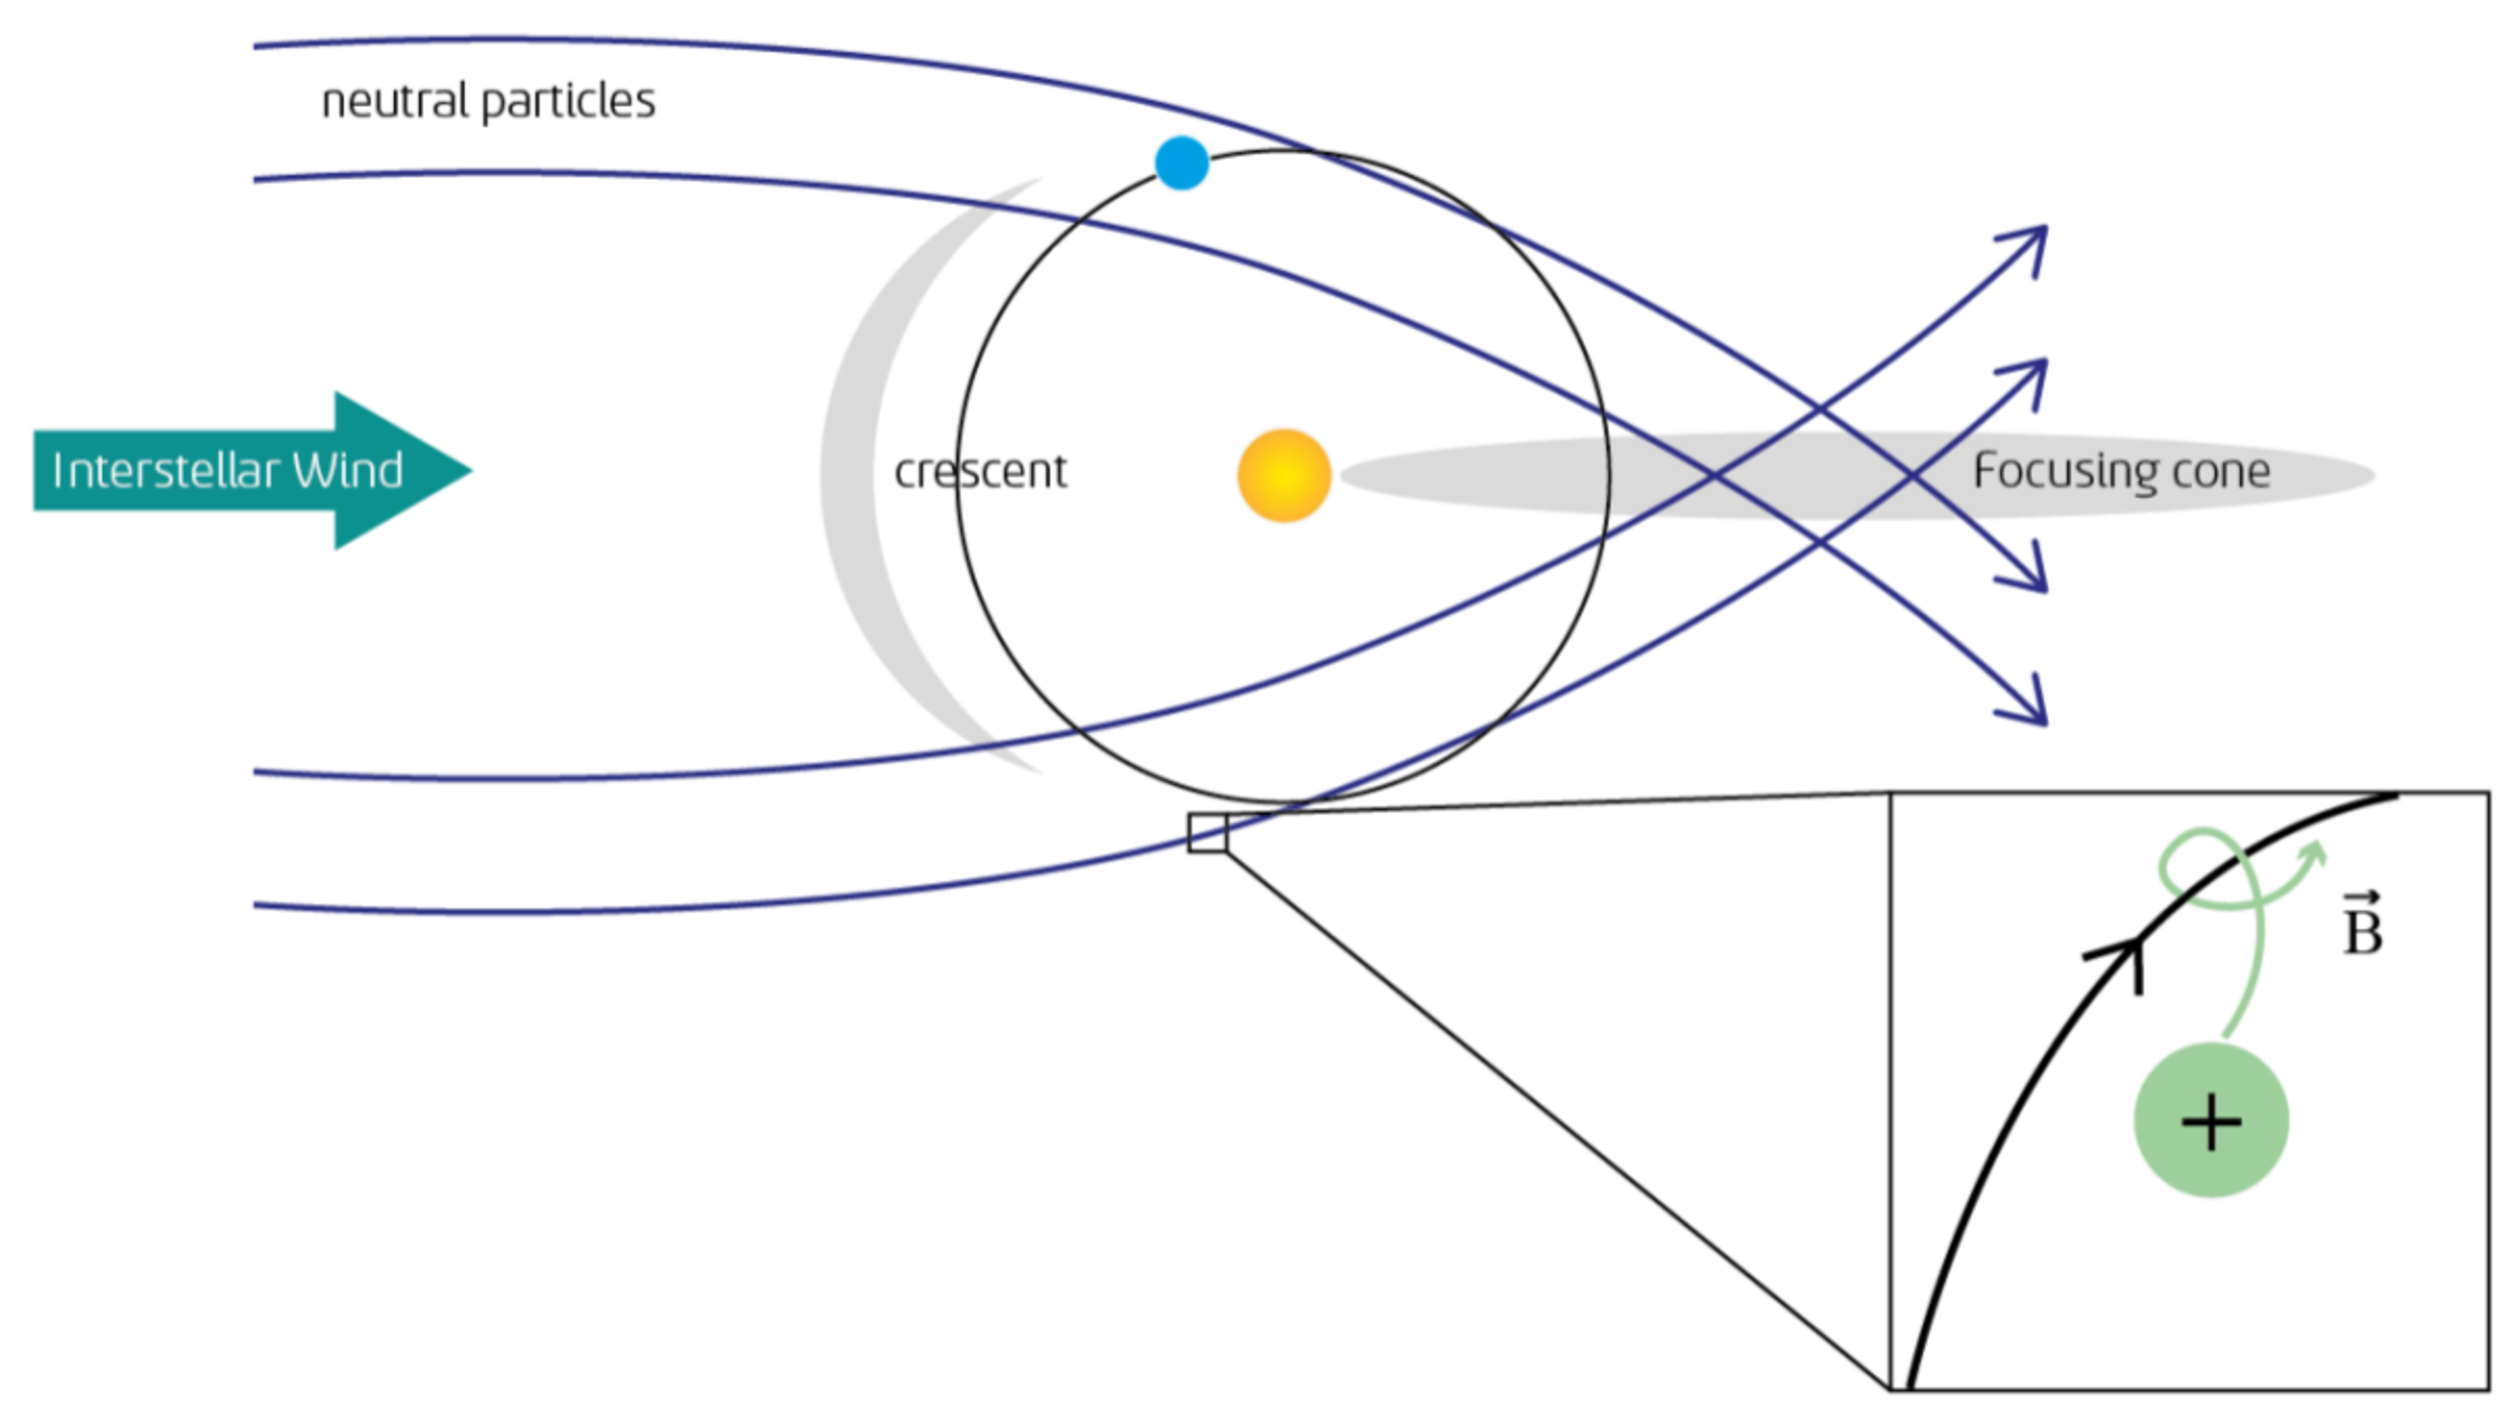
\includegraphics[scale=0.2]{Pics/PU_process.pdf}
	\caption{\begin{flushright}
			\tiny{\textit{Taut, Drews et al., AGU fall meeting 2014}}
	\end{flushright}}
\end{figure}

\end{frame}
%%%
\begin{frame}{PUI -- Measurement}
\begin{columns}
	\column[]{4cm}
	
	\textbf{Observed PUIs:} \\H\textoverscript{1+}, \textoverscript{3}He\textoverscript{1+}, He\textoverscript{1+}, He\textoverscript{2+}, C\textoverscript{1+}, N\textoverscript{1+}, O\textoverscript{1+}, Ne\textoverscript{1+}, Mg\textoverscript{1+}, Si\textoverscript{1+}, Fe\textoverscript{1+}
	
	\vspace{0.7cm}
	%
	\textbf{PUI or Solar Wind?}
	\begin{itemize}
		\item Charge state
		\item Velocity distribution function (VDF)
	\end{itemize}
	
	\column[]{6.5cm}
	\begin{figure}									
		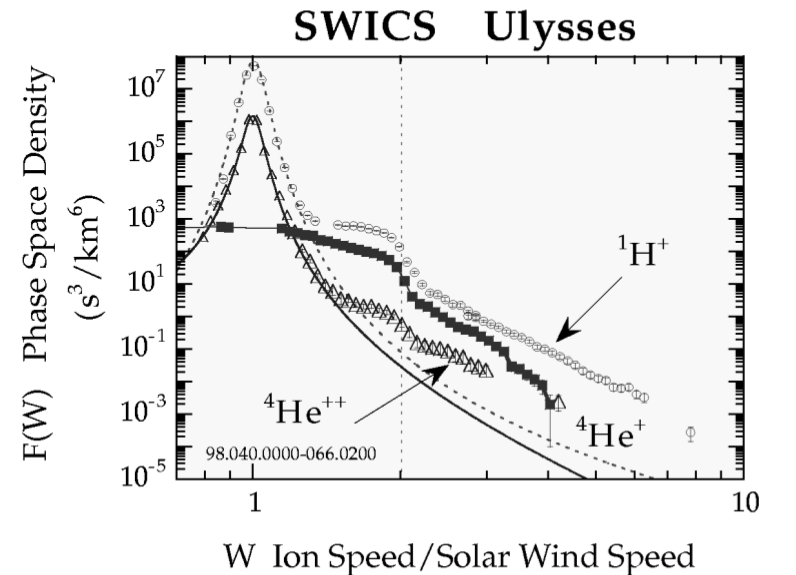
\includegraphics[scale=0.25]{Pics/sw_pui_gloeckler.png}
		\caption{\begin{center}\tiny{Gloeckler et al., 1999}
		\end{center}}
	\end{figure}
\end{columns}
\end{frame}
%%%



%
%
%

\begin{frame}{The Pickup Process}
	\begin{columns}
		\column{5.5cm}
		\vspace{0.5cm}
		\flushright
		\begin{figure}
			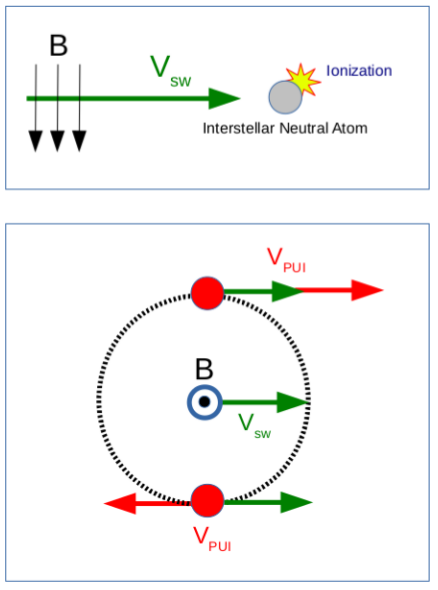
\includegraphics[scale=0.3]{Pics/pu_process_1_2.png}
			%\hspace{1cm}
			\caption{\begin{center}
					\tiny{Taut, Drews et al., AGU Fall Meeting 2014}
			\end{center}}
		\end{figure}
		\column{5cm}
					
			\begin{center}
				\textbf{Velocity Space:}
			\end{center}
			%\vspace{0.5cm}
			\begin{figure}									
				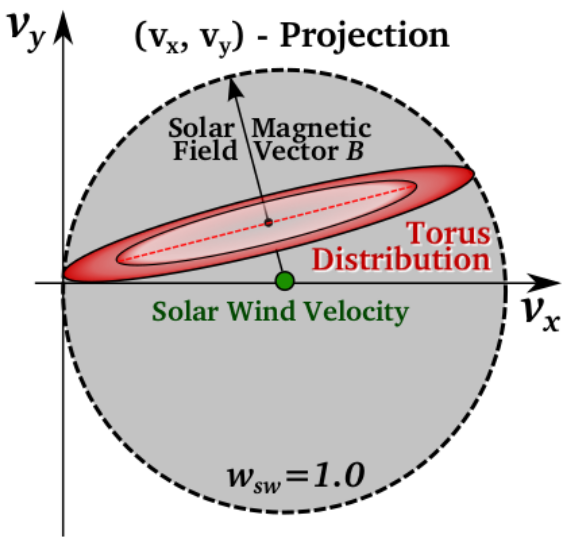
\includegraphics[scale=0.22]{Pics/injiz.png}
				\caption{\tiny{\begin{center}
							\textit{Drews et al., 2016}
				\end{center}}}
		\end{figure}
	\vspace{-1cm}
				\begin{center}
					\textbf{$\rightarrow$ Anisotropic torus VDF}	
				\end{center}
	\end{columns}
\end{frame}
%
%
%
\begin{frame}{Evolution of the VDF}
	\begin{figure}
		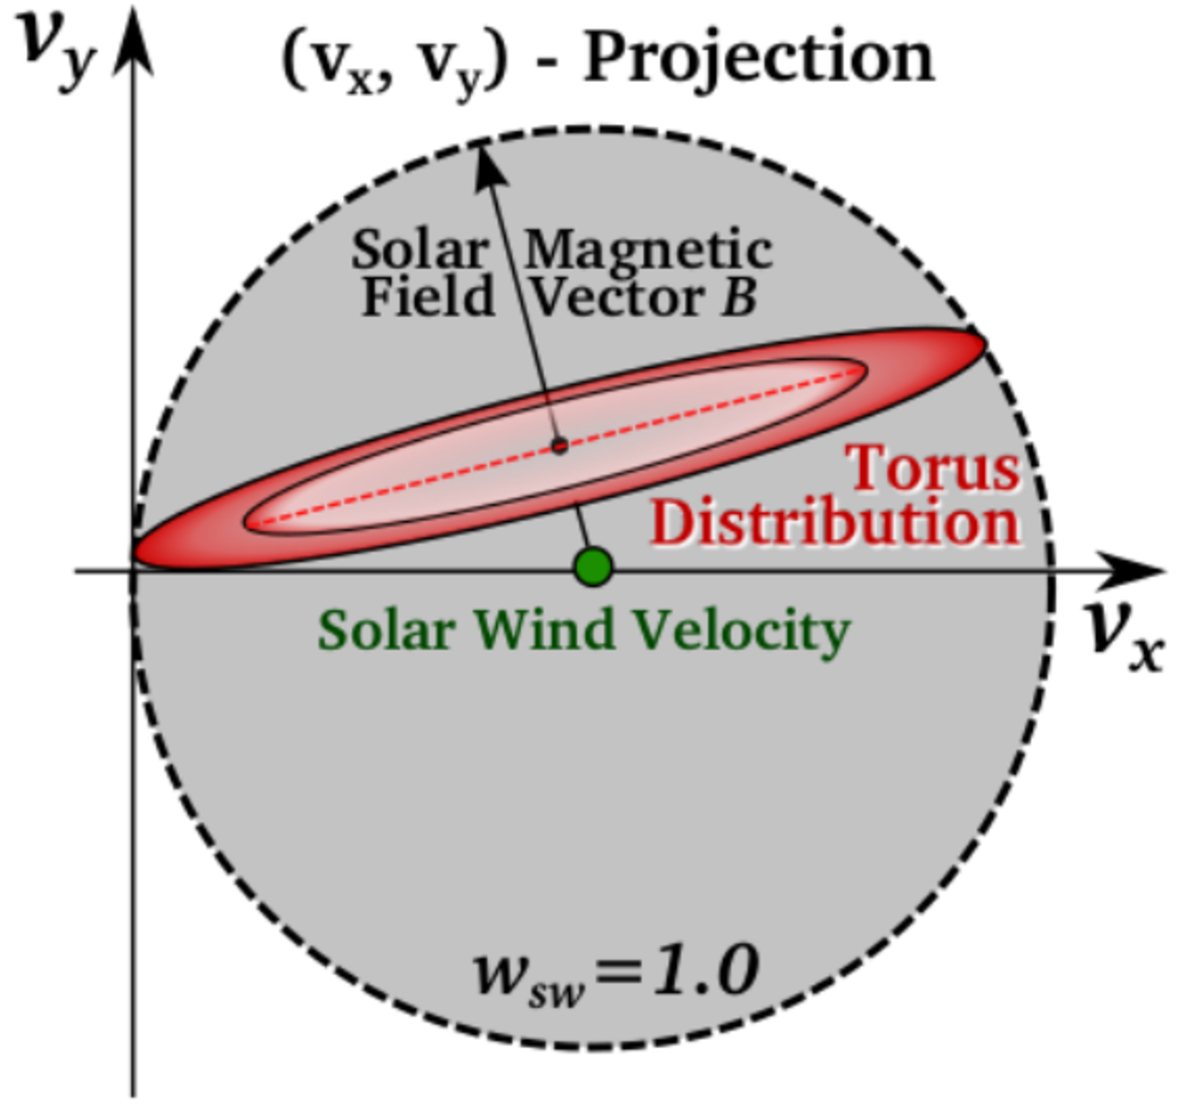
\includegraphics[scale=0.17]{Pics/torus.pdf}
		\hspace{0.001cm}
		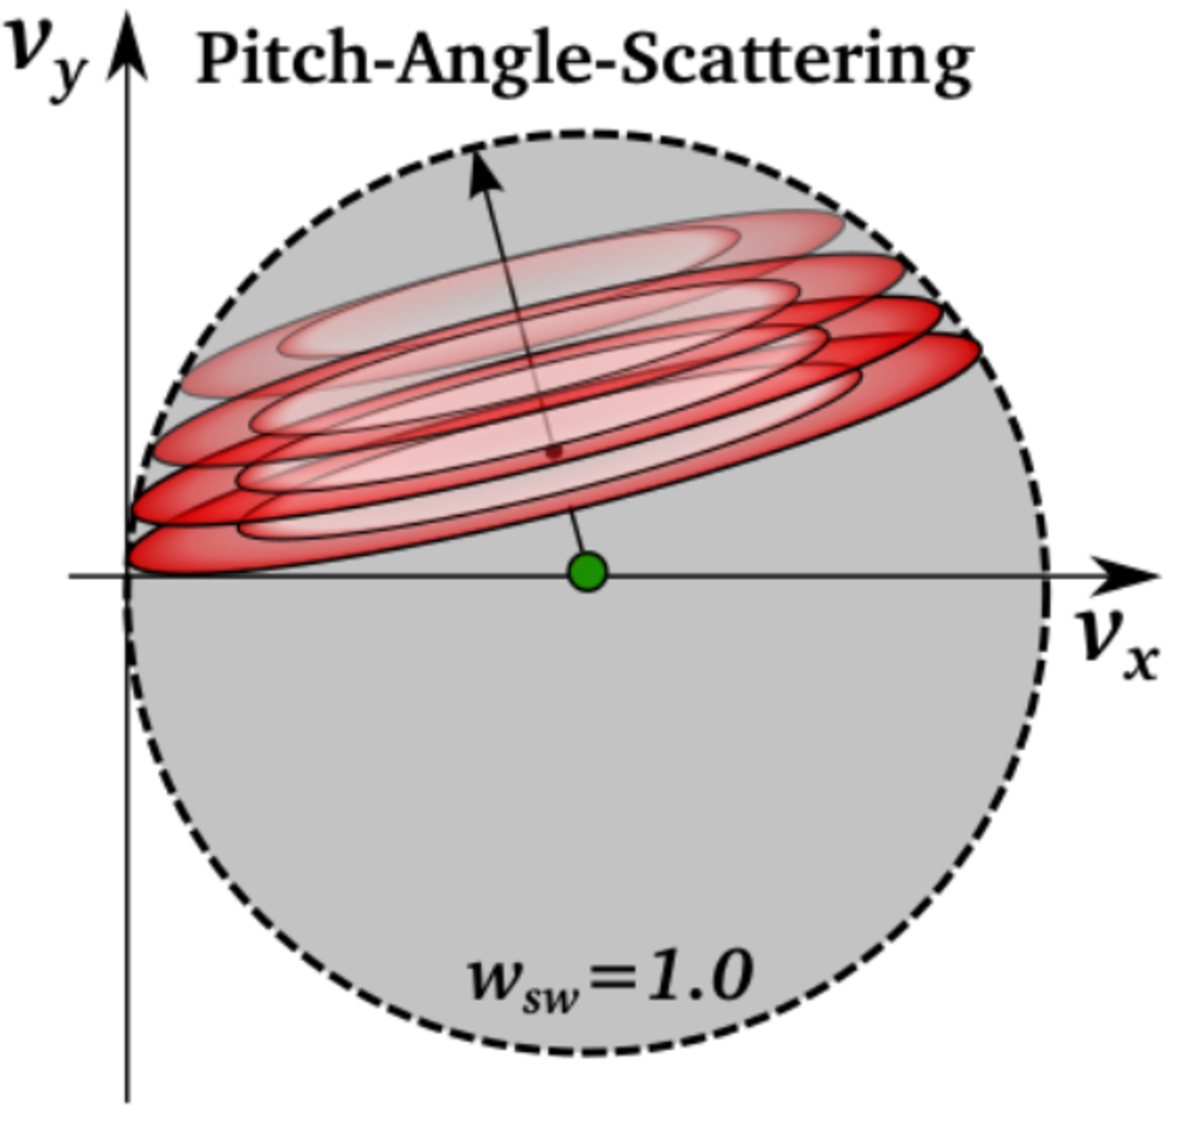
\includegraphics[scale=0.17]{Pics/PAS.pdf}
		\hspace{0.001cm}
		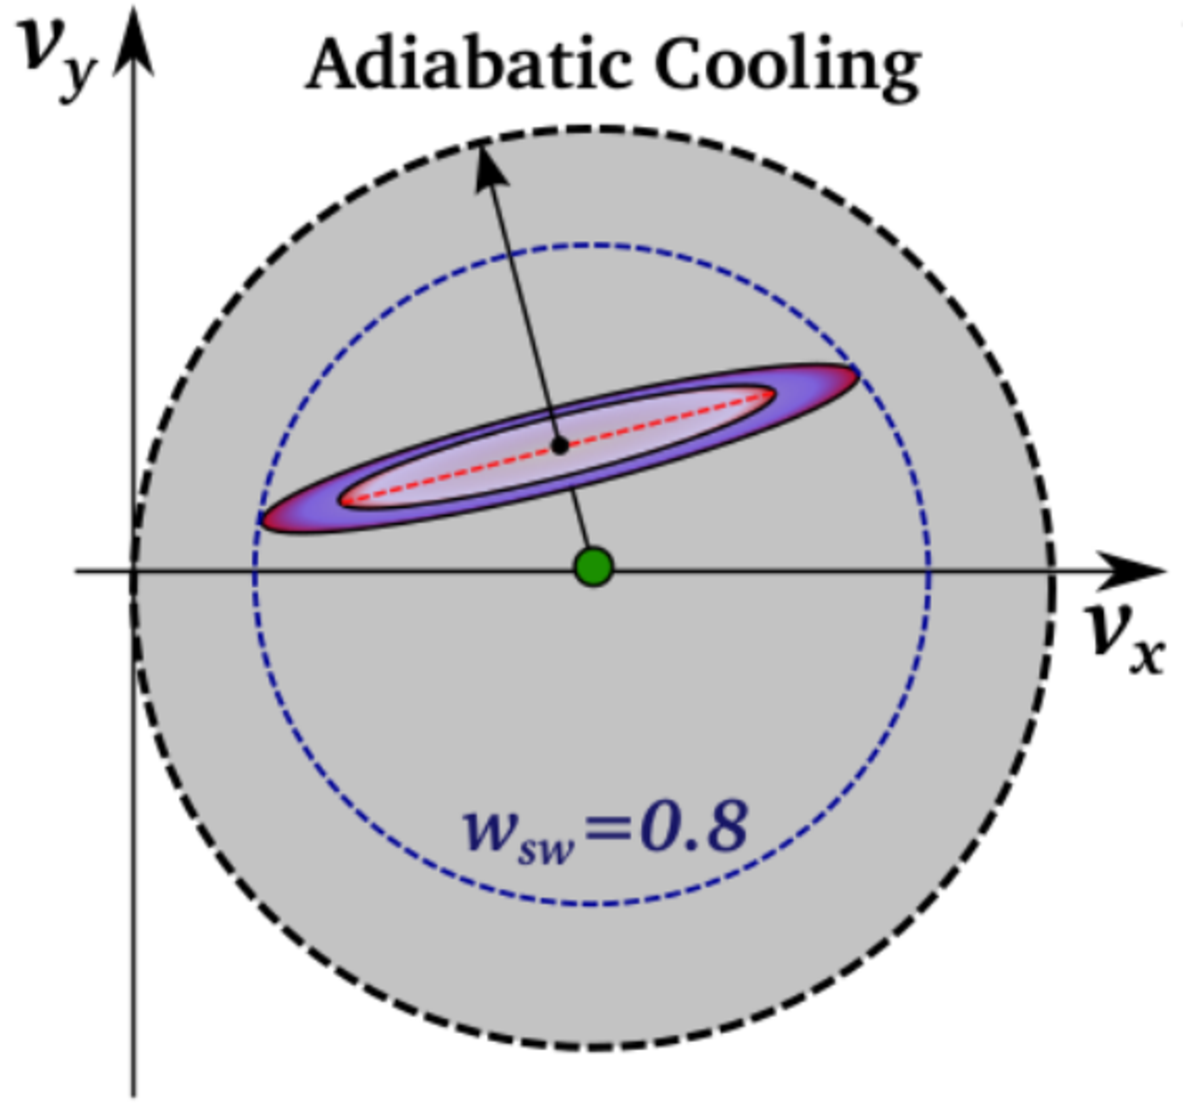
\includegraphics[scale=0.17]{Pics/Cooling.pdf}
		\vspace{0.5cm}
		\caption{\tiny{\begin{flushright}
					\textit{Drews, Berger et al., 2016}
		\end{flushright}}}
	\end{figure}
	\vspace{-.5cm}
	\begin{columns}
		\vspace{.5cm}
		\column{4cm}
		Modification of the initial torus-shaped VDF by:
		\column{6cm}
		\begin{itemize}
			\item Pitch-angle scattering \\ $\rightarrow$ isotropisation
			\item acceleration \& deceleration
		\end{itemize}
	\end{columns}
%
%	
%	
\end{frame}

%



\begin{frame}{Anisotropic features of the VDF}
\begin{columns}
	\column[]{.2cm}
	\hspace{-1cm}
	\column[]{5.cm}
	\vspace{1.1cm}
	\begin{figure}									
		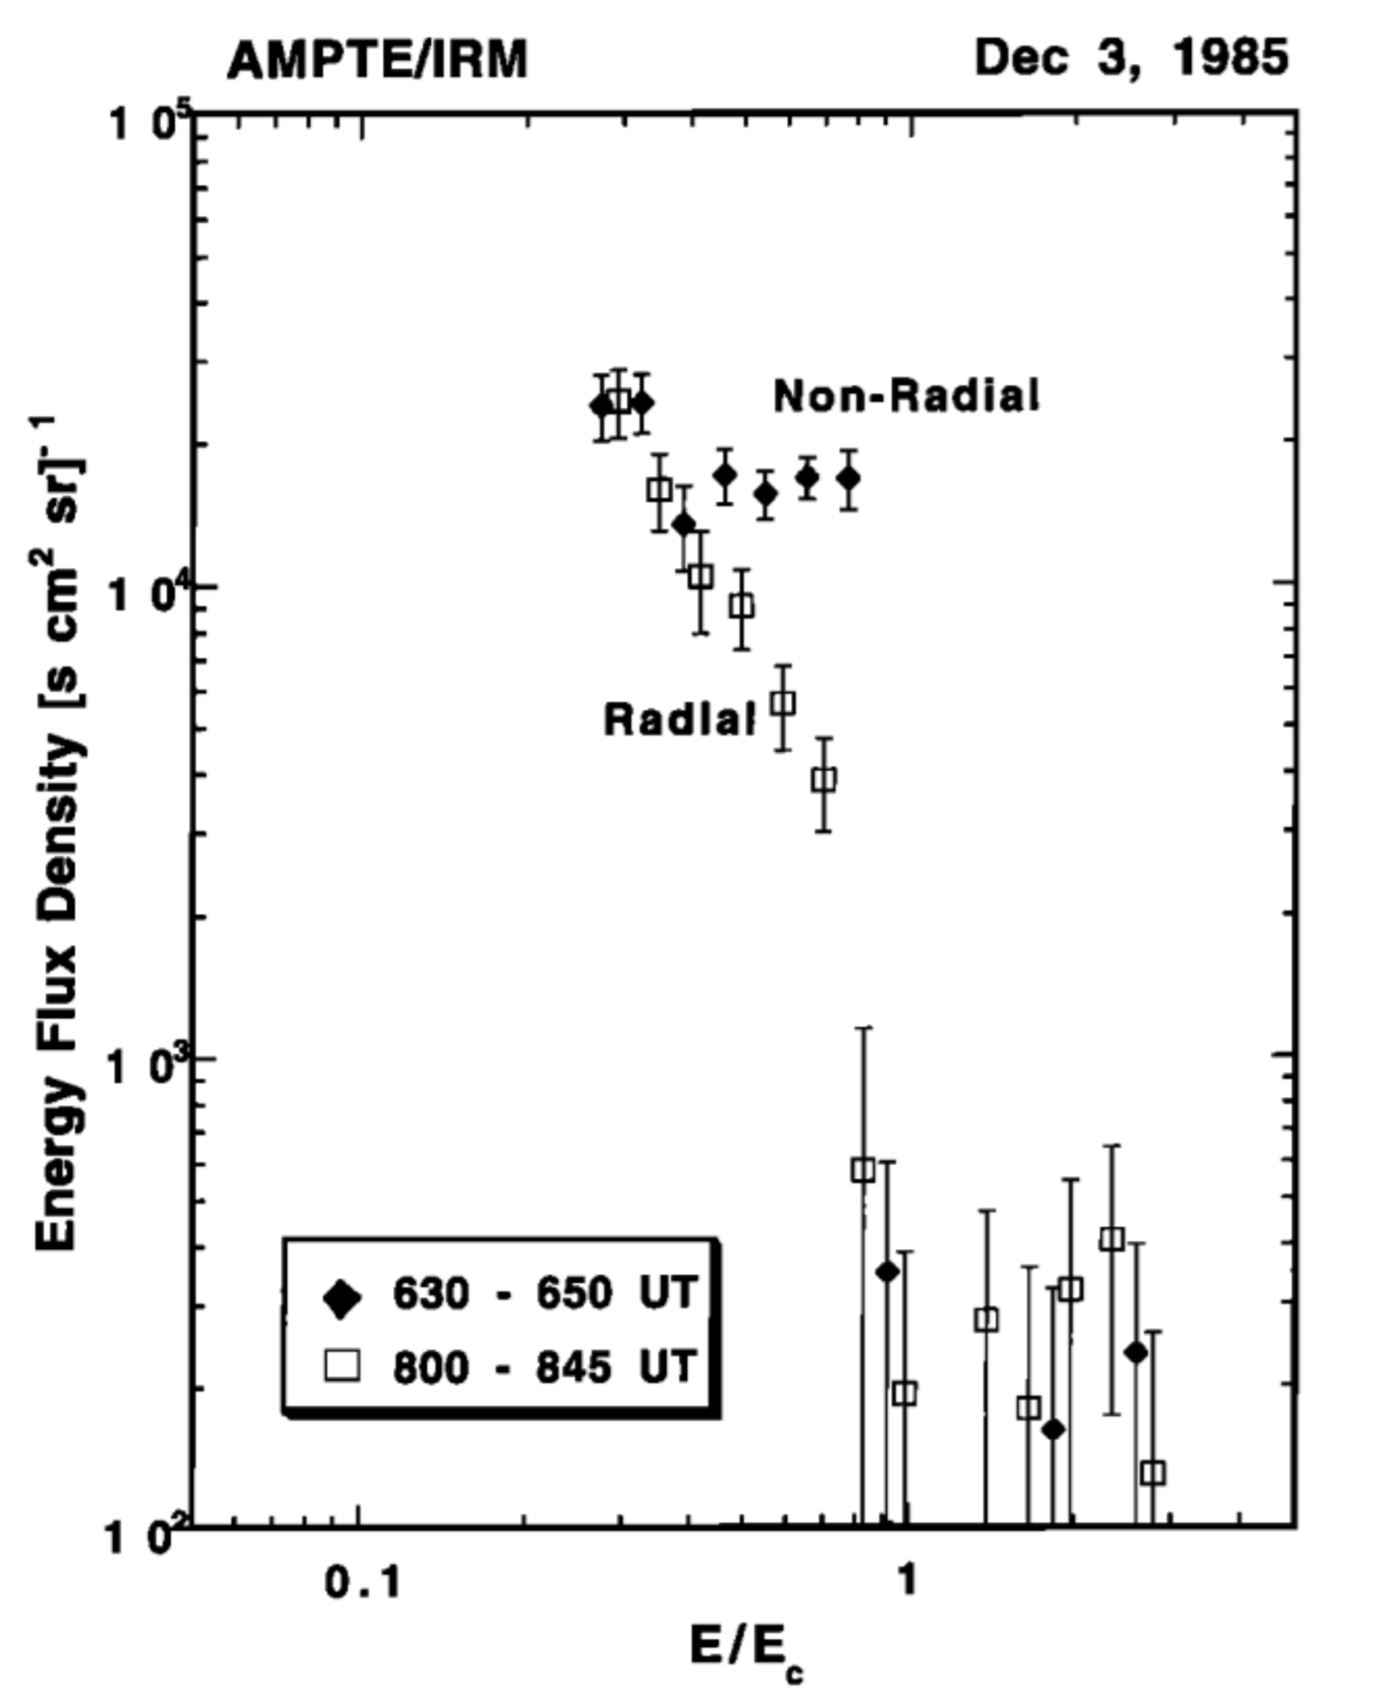
\includegraphics[scale=0.2]{Pics/moebius_dec.pdf}
		\caption{\begin{center}\tiny{Moebius et al., 1998}
		\end{center}}
		
	\end{figure}
	\column[]{7cm}
	\begin{figure}
										
		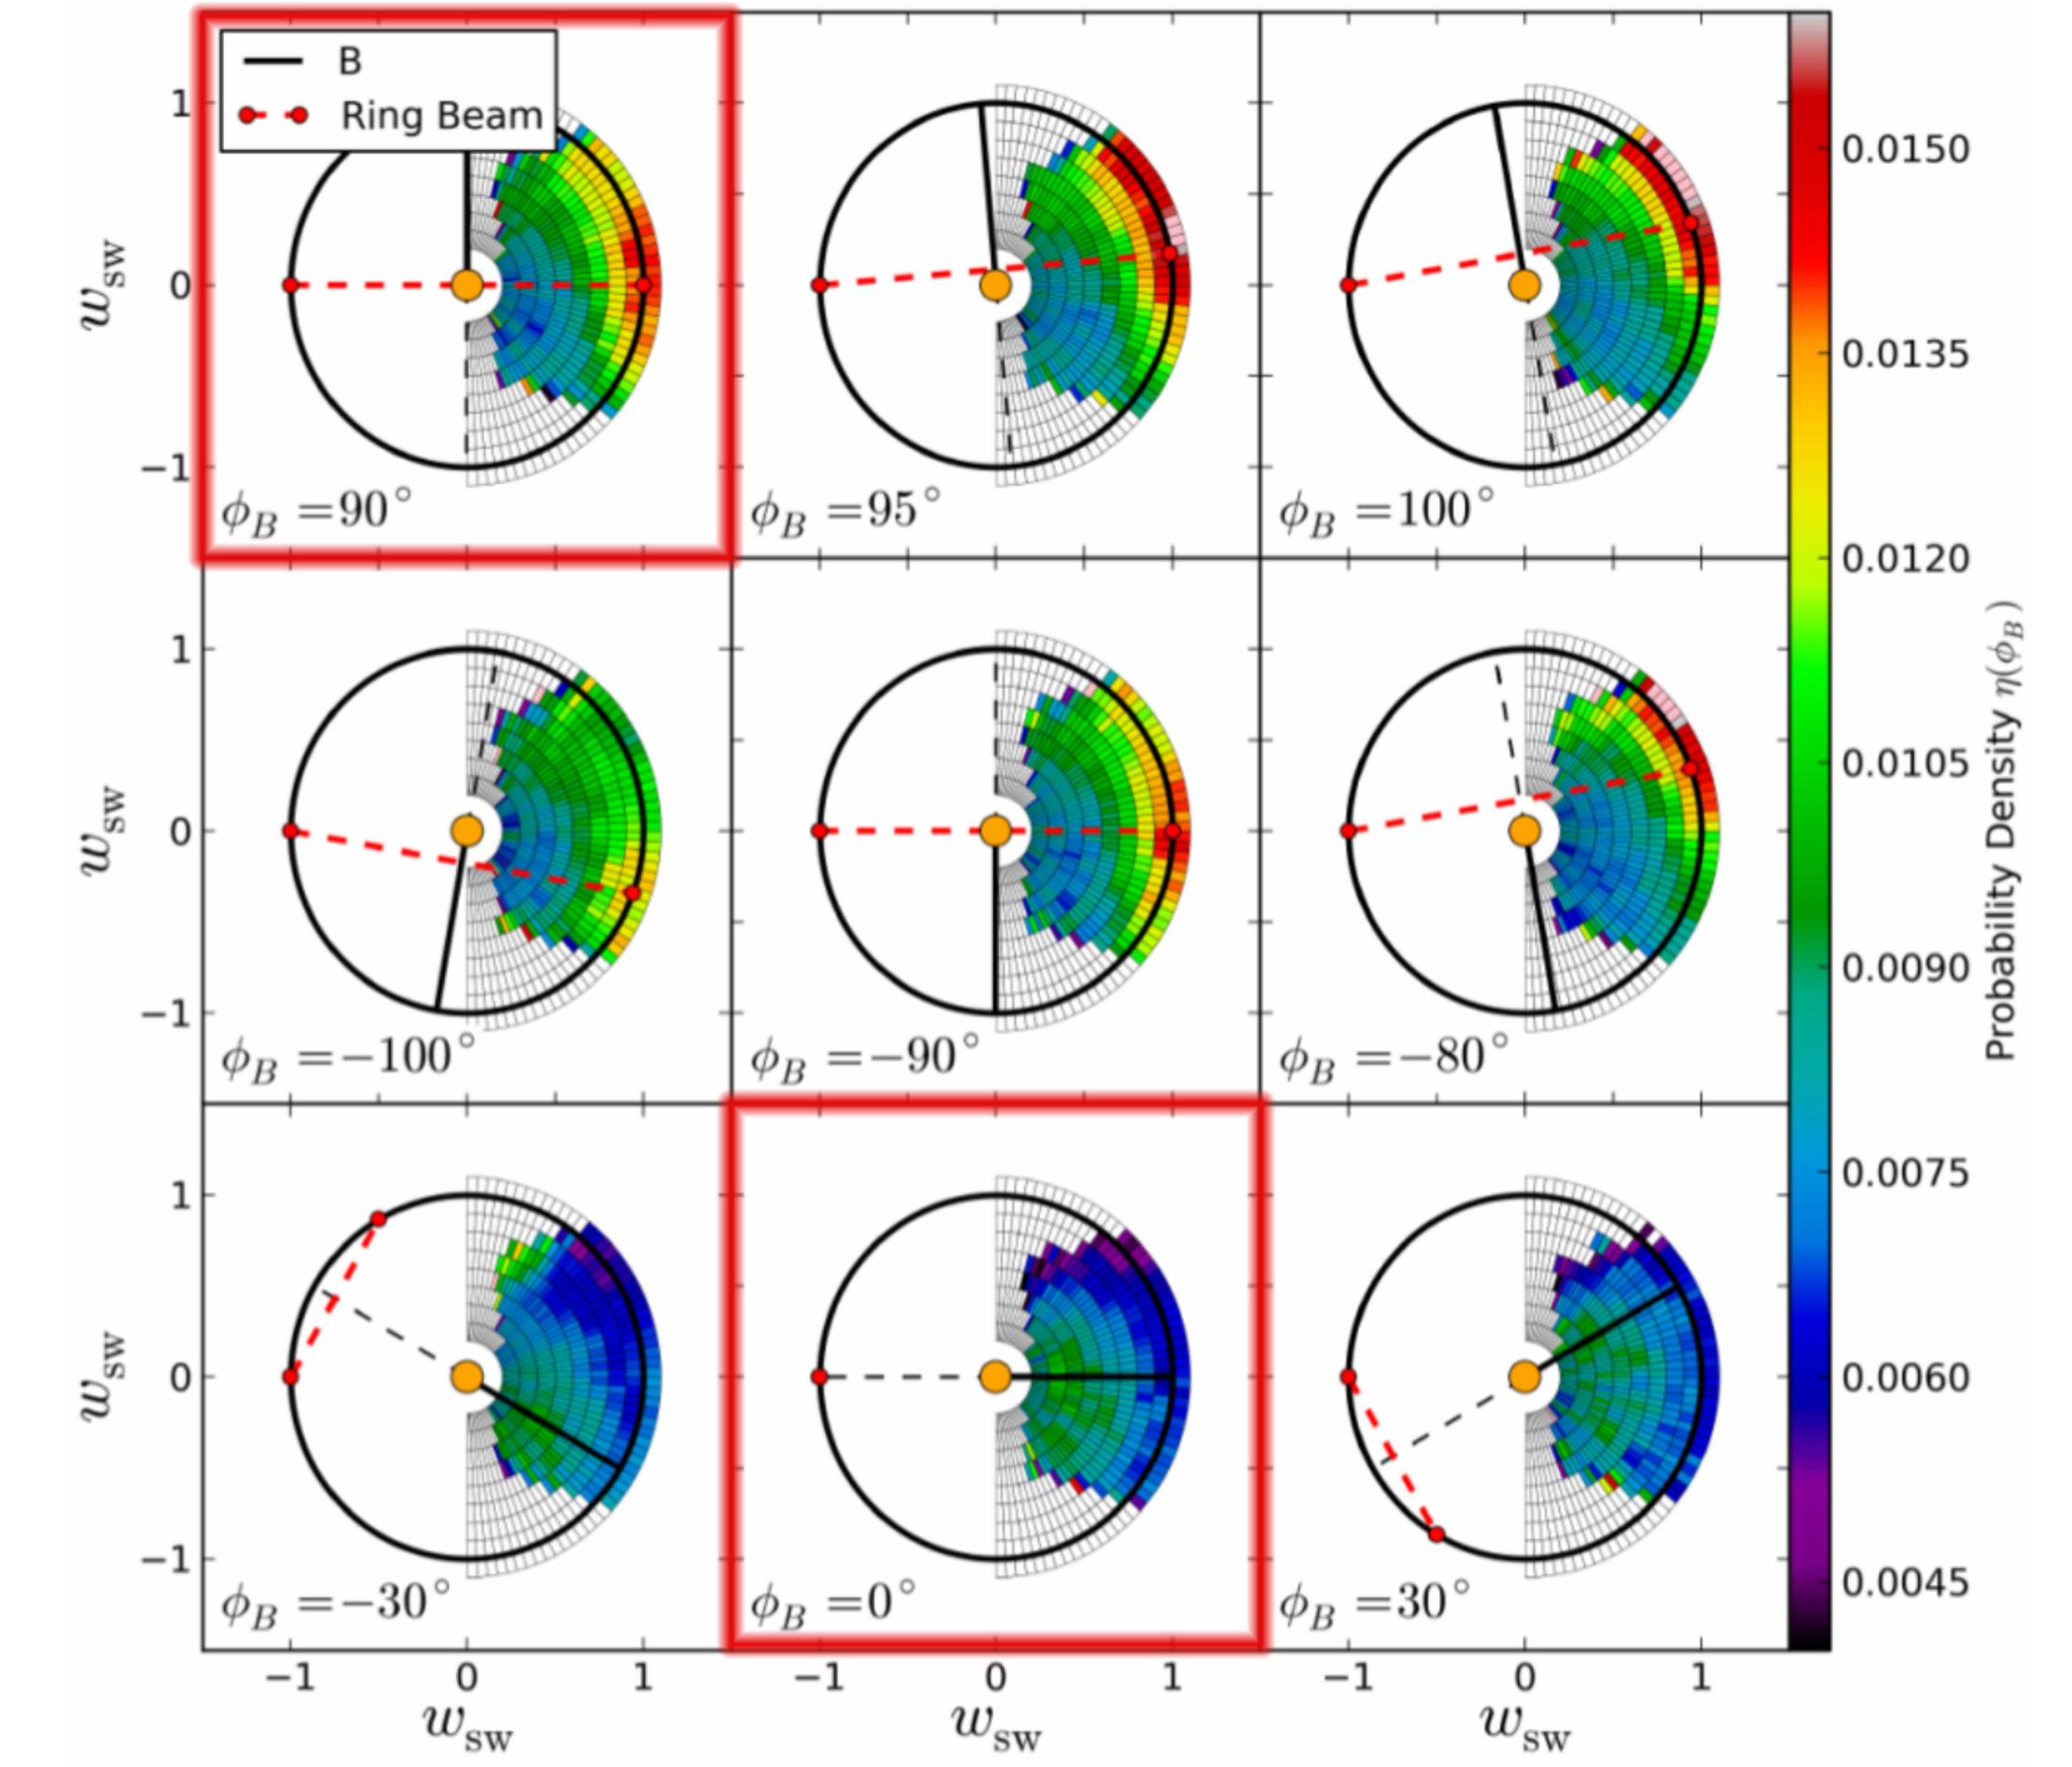
\includegraphics[scale=0.2]{Pics/rvdf_9er_framed.pdf}
		\caption{\tiny{\begin{center}
					\textit{Drews, Berger et al., 2015}
		\end{center}}}
	\end{figure}
\column[]{.5cm}
\end{columns}
\end{frame}



\section{Motivation}
\begin{frame}{Motivation}
\begin{columns}
	\column[]{5cm}
	Problem: \\ Ambiguity of 1D reduced data
	\\[1cm]
	For fully understanding the PUI transport in phase space we need to analyse the \textbf{3D velocity distribution} function
%	GRUNDSÄTZLICHES PROBLEM
%	warum 3d?
%	\begin{itemize}
%		\item Uneindeutigkeit der reduzierten 1D-Daten (unendlich viele Modellfunktionen)
%		\item einzelne Prozesse können nicht unterschieden werden
%		\item Übergang SW-frame
%	\end{itemize}
	
	\column[]{5cm}
	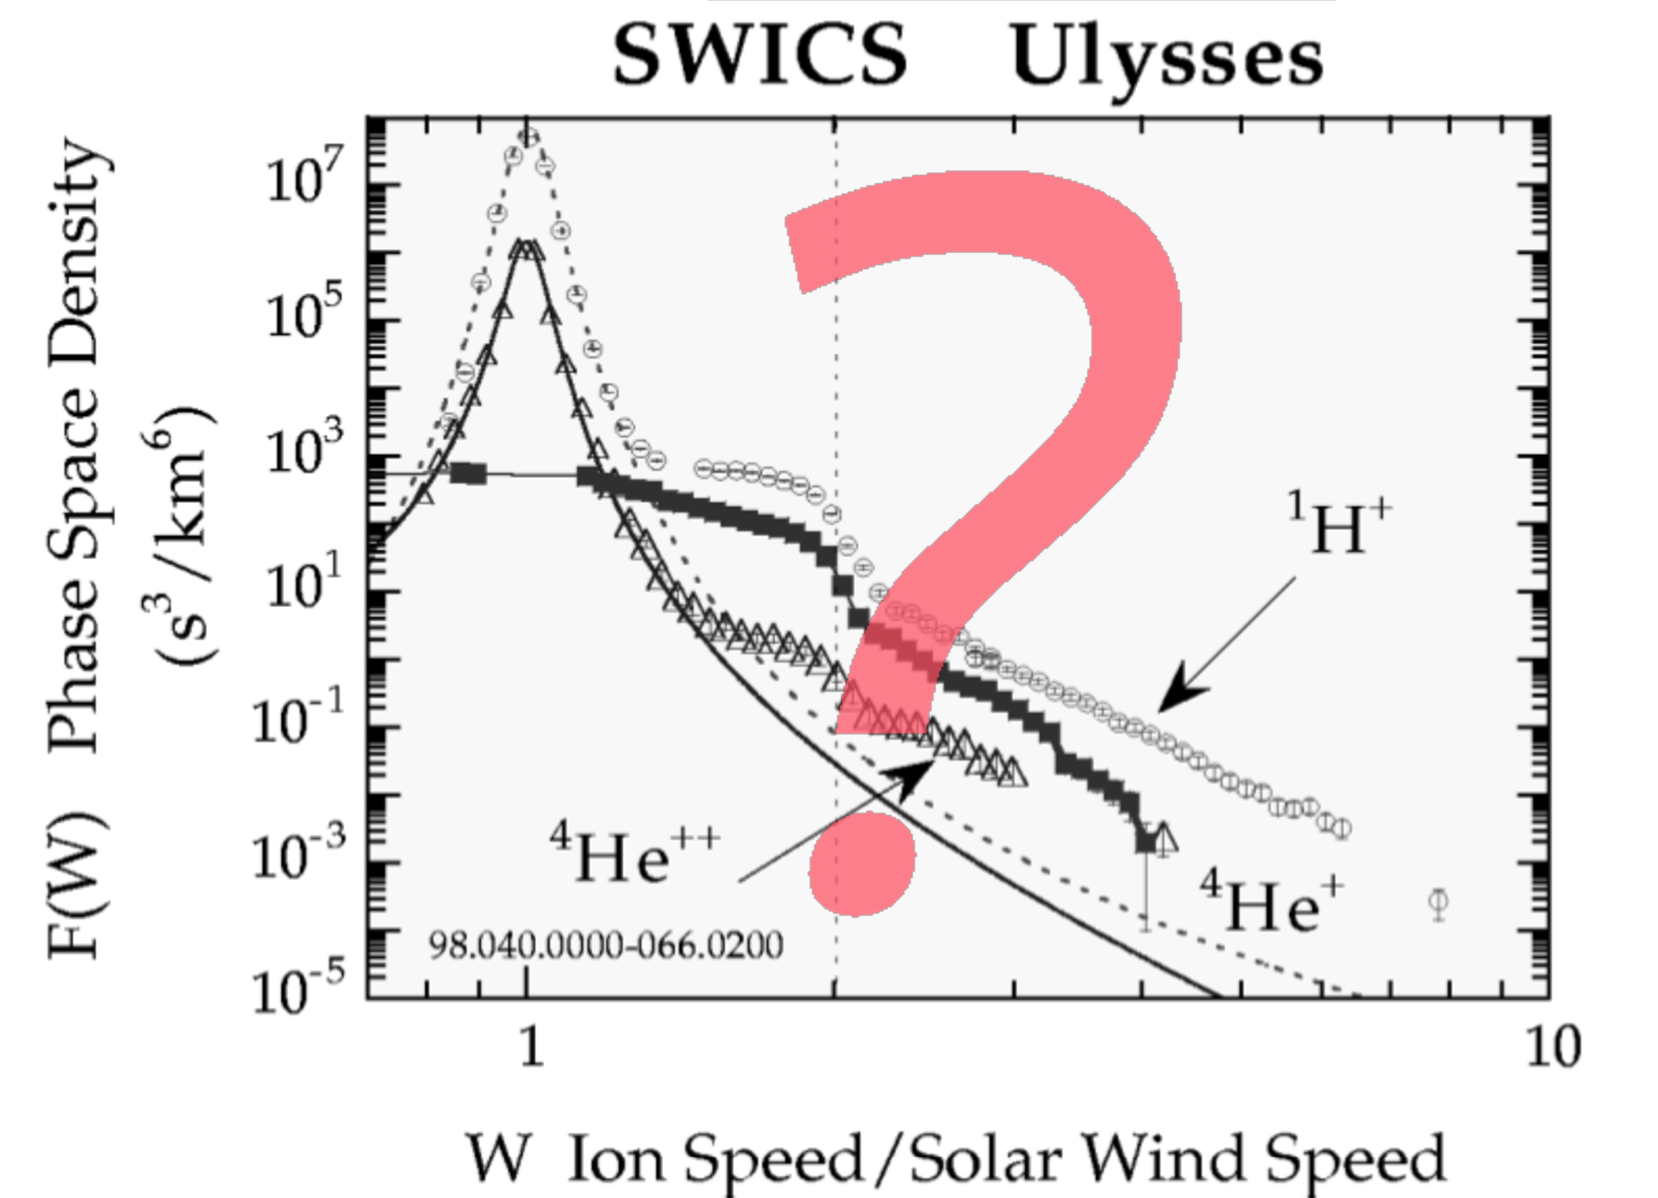
\includegraphics[scale=0.18]{Pics/qm.pdf}
\end{columns}

\end{frame}
%%%

%%%

\begin{frame}{Frame of Reference}
\begin{columns}
	\column[]{5cm}
	\vspace{-1cm}
	\begin{figure}
		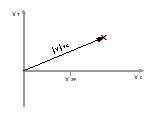
\includegraphics[scale=2.2]{Pics/vspace_sc_trans.pdf}
	\end{figure}
	\vspace{-1.2cm}
	\begin{figure}
		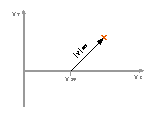
\includegraphics[scale=2.2]{Pics/vspace_sw_trans.pdf}
	\end{figure}
	
	
	\column[]{6.2cm}
	\vspace{.5cm}
	\begin{figure}
		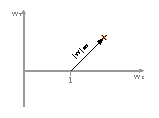
\includegraphics[scale=2.2]{Pics/wspace_sw_trans.pdf}
	\end{figure}
\end{columns}
\end{frame}

%%%

%
%
%

\section{Ulysses SWICS}
\begin{frame}{Ulysses Spacecraft (1990 -- 2009)}

\begin{figure}
	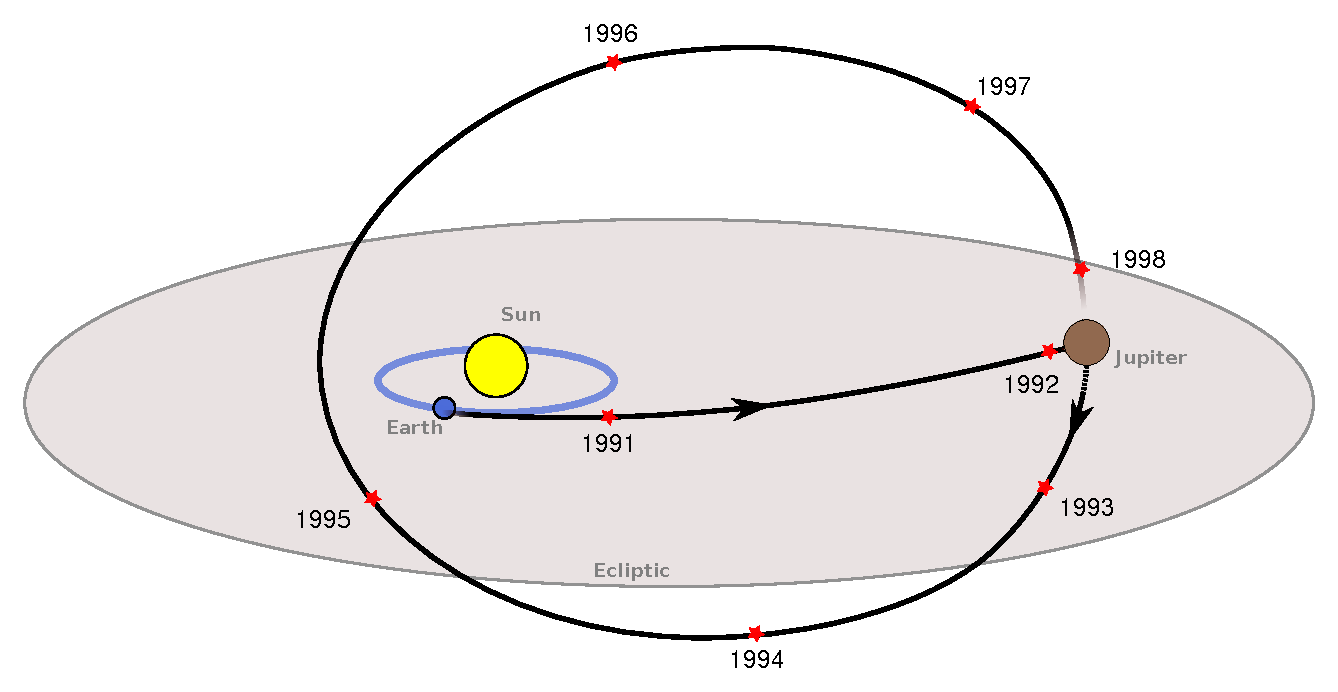
\includegraphics[scale=0.4]{Pics/ulysses_trajectory.pdf}
	\caption{\tiny{\begin{center}
				\textit{adapted from www.cosmos.esa.int, 2019}\end{center}}}
\end{figure}

	
\begin{columns}
	\column[]{4.8cm}
	\vspace{-1cm}
	\begin{itemize}
		\item Highly inclined orbit;\\ orbital period: 6.2 years
		\item spin-stabilized
	\end{itemize}

	\column[]{5.5cm}
	\vspace{-1cm}
	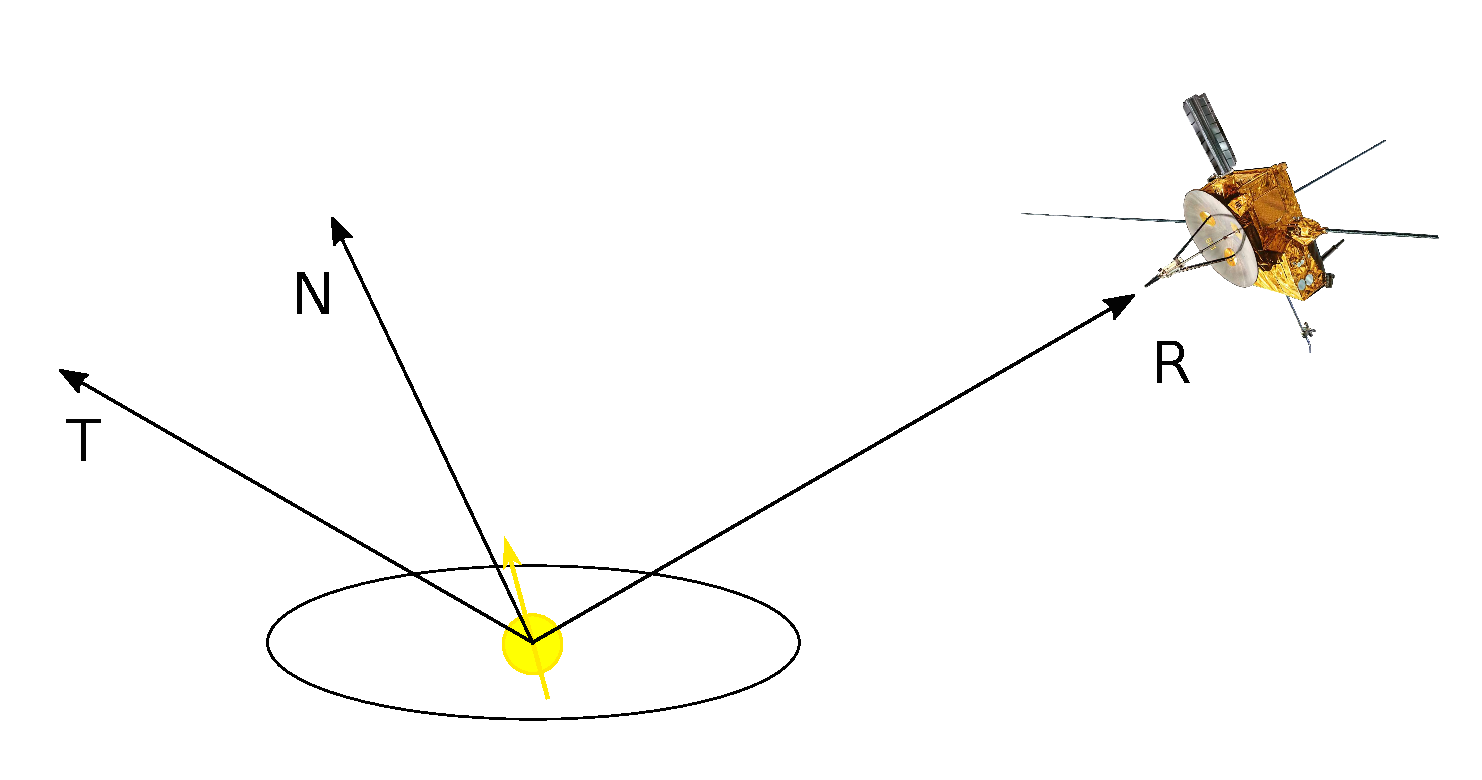
\includegraphics[scale=0.25]{Pics/RTN.pdf}
\end{columns}

\end{frame}









%%%
\begin{frame}{SWICS}
	
	\begin{columns}
		
		\column[]{4cm}
		\small{The \textbf{S}olar \textbf{W}ind \textbf{I}on \textbf{C}omposition \textbf{S}pectrometer} \\
		
		\begin{itemize}
			\item Time-of-flight mass spectrometer
			\item $\left\{\frac{E}{q}, ToF, E_{SSD}\right\}$ $\Rightarrow \left\{\frac{M}{q}, M, |v|\right\}$ 
			\item identification \& energy of the ion 
		\end{itemize}

		
		\column[]{6.4cm}
		\begin{figure}
			\hspace{2cm}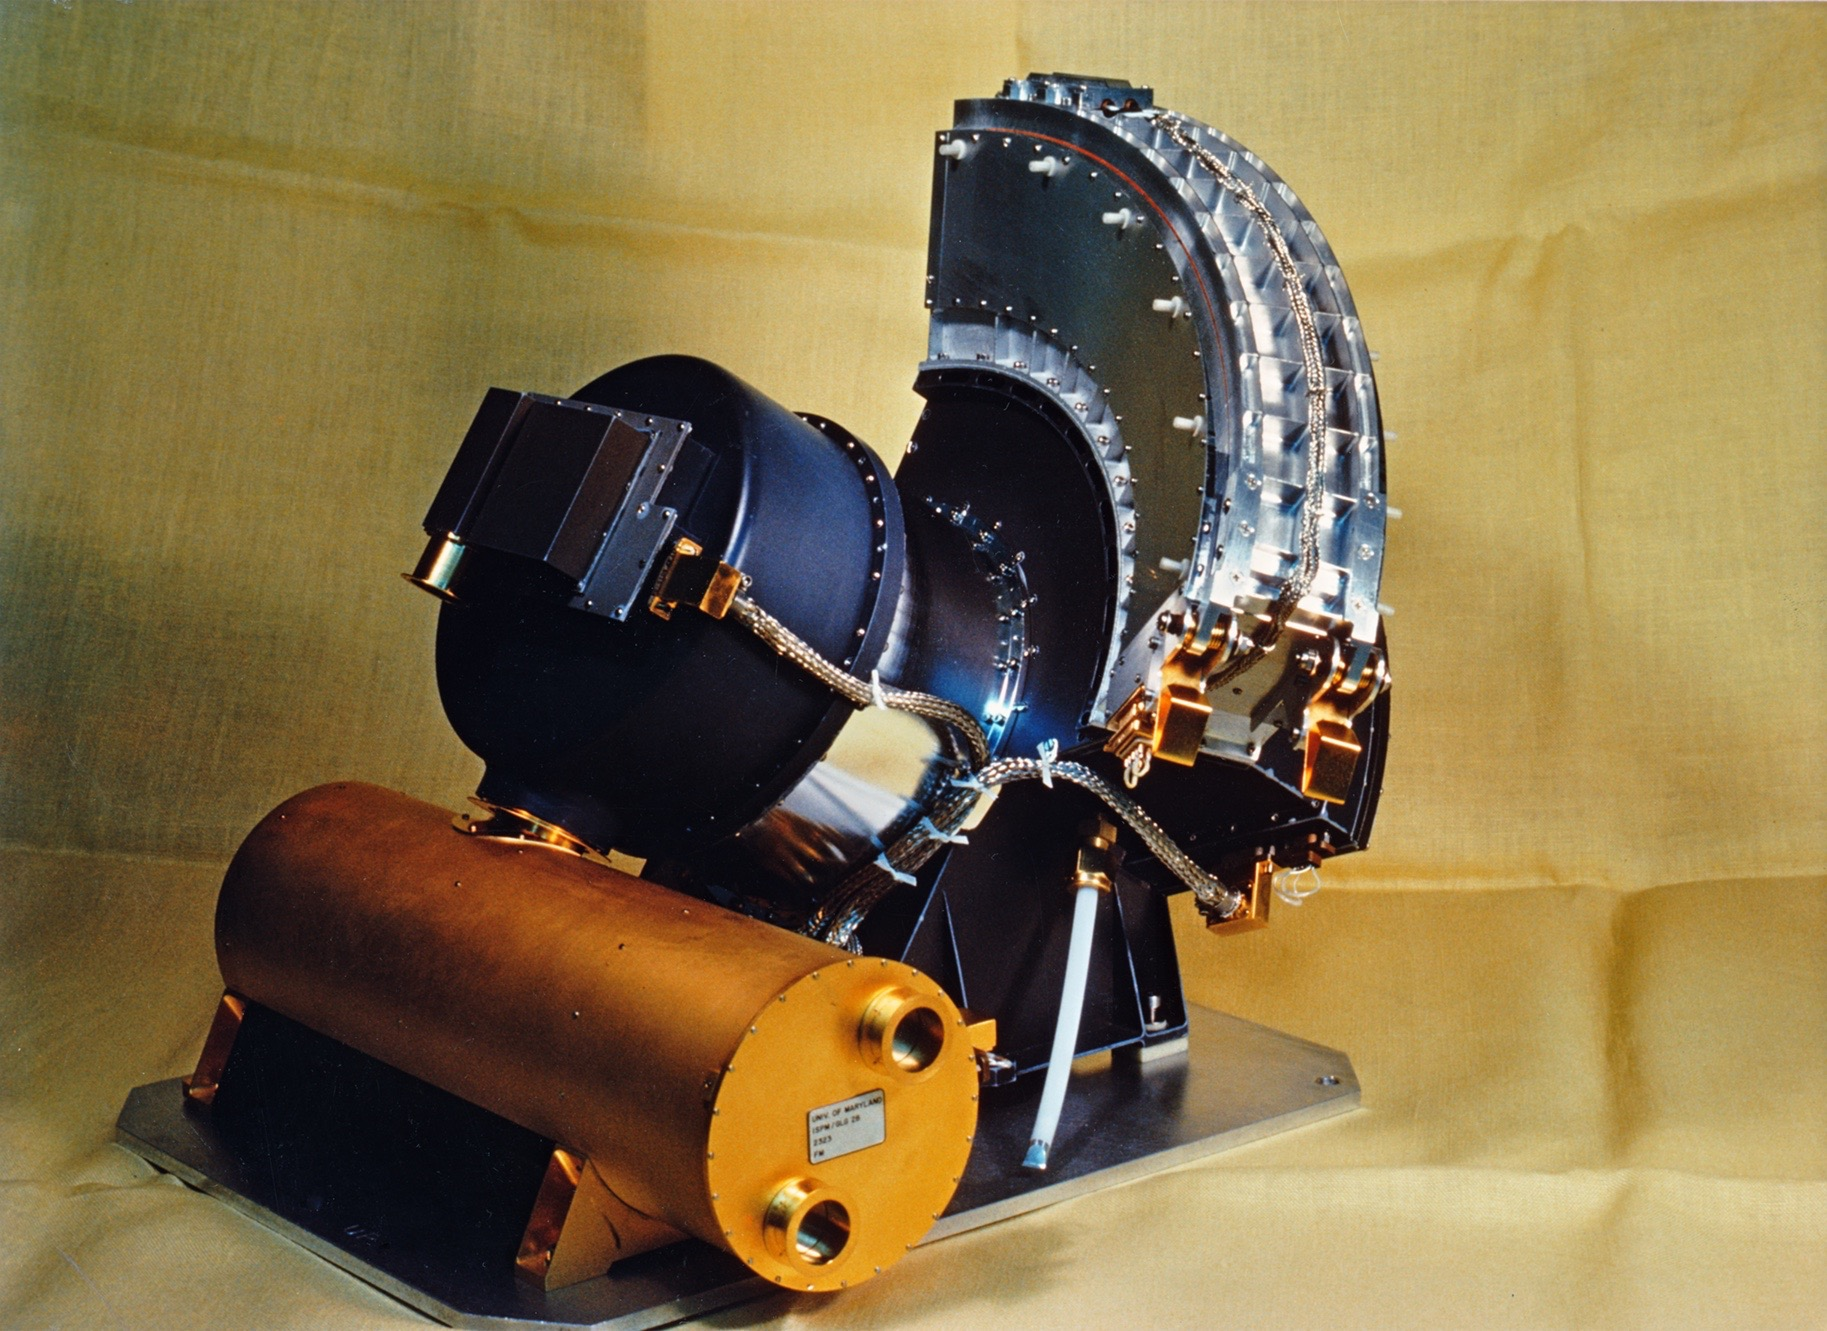
\includegraphics[scale=0.06]{Pics/ULYSSES-SWICS.jpg}
			\vspace{0.1cm}							
			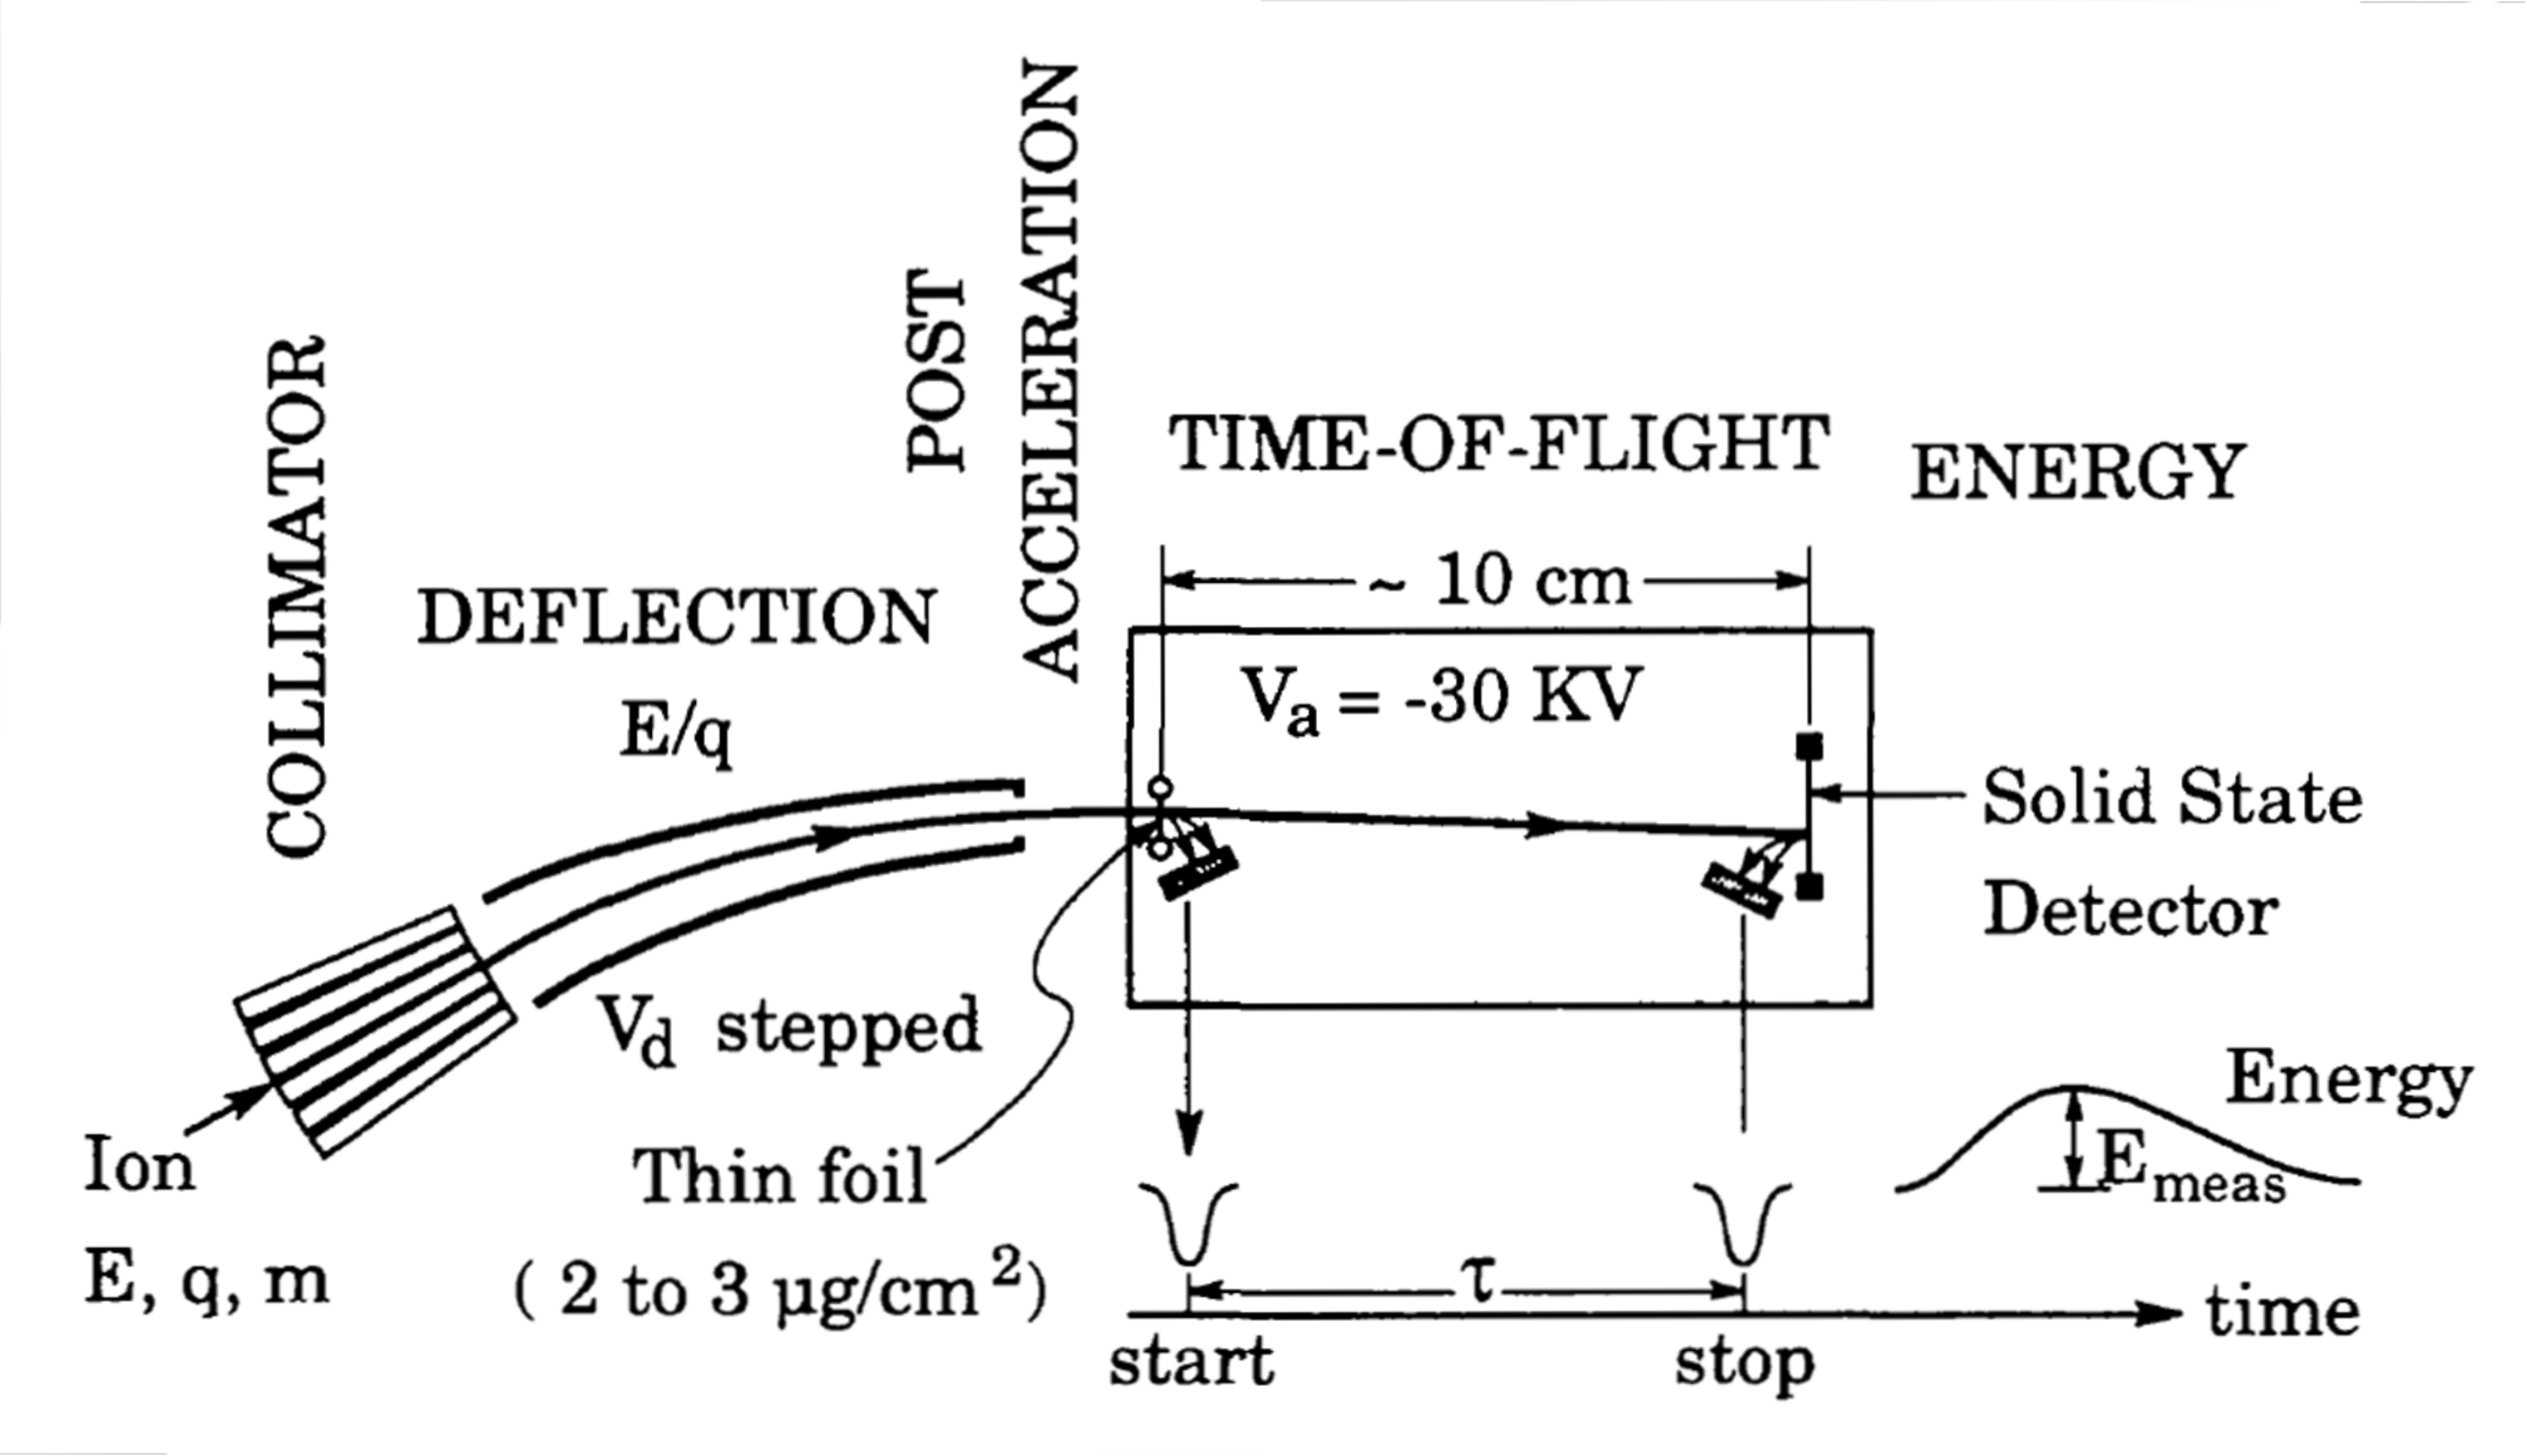
\includegraphics[scale=0.15]{Pics/SWICS_measurement_gerade.pdf}
			\caption{\tiny{\begin{center}
						\textit{Gloeckler, Geiss et al., 1992}\end{center}}}
		\end{figure}
		
	\end{columns}
\end{frame}



%%%
\begin{frame}{PHA data}
\vspace{0.8cm}
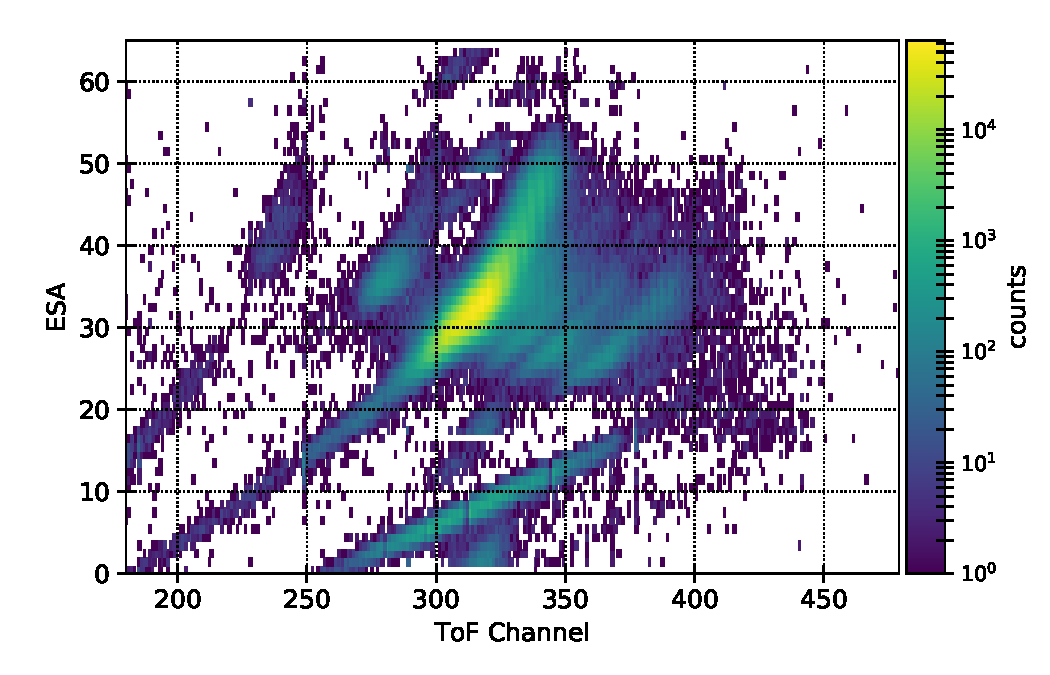
\includegraphics[scale=0.65]{Pics/epq_rng0.pdf}
\begin{columns}
	\column{1.1cm}
	\column{3.4cm}
	\vspace{-15.8cm}
	\begin{mdframed}[roundcorner=4pt,userdefinedwidth=3cm,
		align
		=center,
		linecolor
		=black,backgroundcolor=blue!8,
		linewidth
		=1pt]
		$\boldsymbol{\frac{E}{q} = \frac{1}{2} \, \frac{m}{q} \, v^2}$
	\end{mdframed}
	
	\column{3.4cm}
	\vspace{-15.8cm}
	\begin{mdframed}[roundcorner=4pt,userdefinedwidth=3.5cm,
		align
		=center,
		linecolor
		=black,backgroundcolor=blue!8,
		linewidth
		=1.pt]
		$\left[\frac{m}{q}\right]_{He^+} = 4 \frac{amu}{C}$
	\end{mdframed}
	\column{1.cm}
\end{columns}
\vspace{-1.0cm}
\end{frame}


%%%
\begin{frame}{EpQ measurement}
	\vspace{-.2cm}
	\begin{columns}
		\column{4.5cm}
		\begin{figure}									
		\only<1,2>{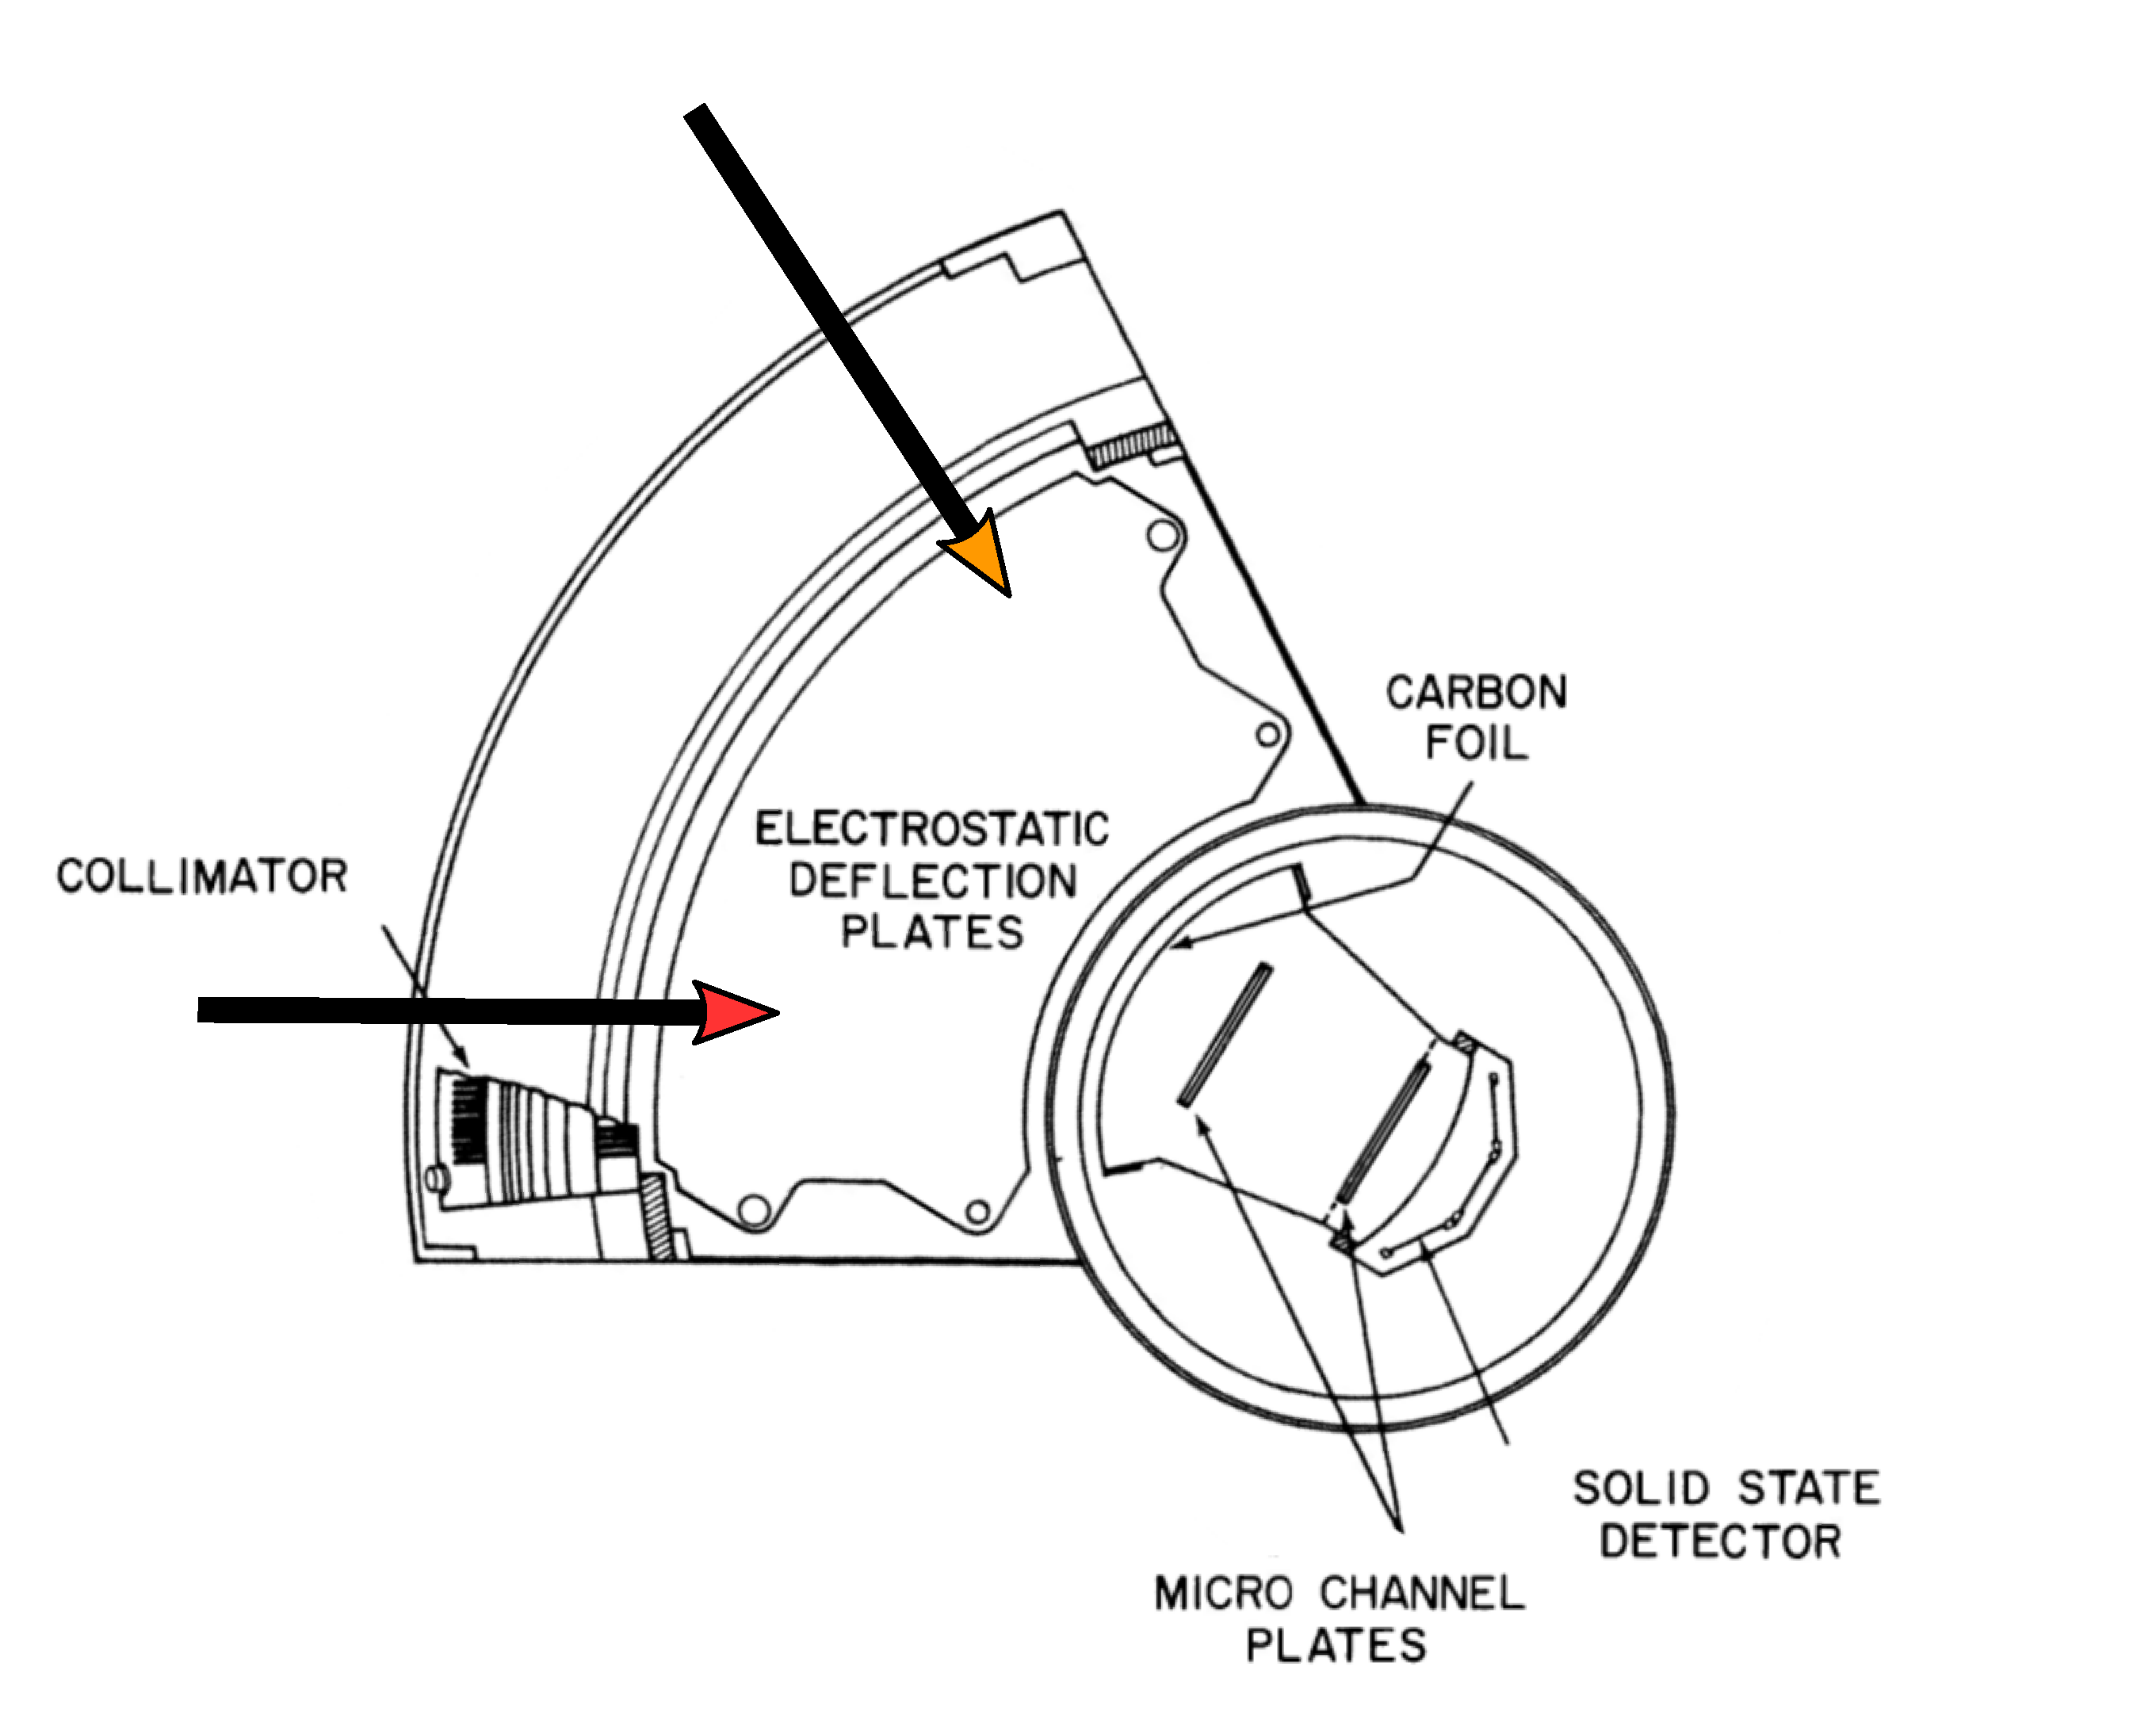
\includegraphics[scale=0.14]{Pics/swics_sensor_flipped_rotated_arrows.pdf}} 

		\end{figure}
		\column{4cm}
		\only<1>{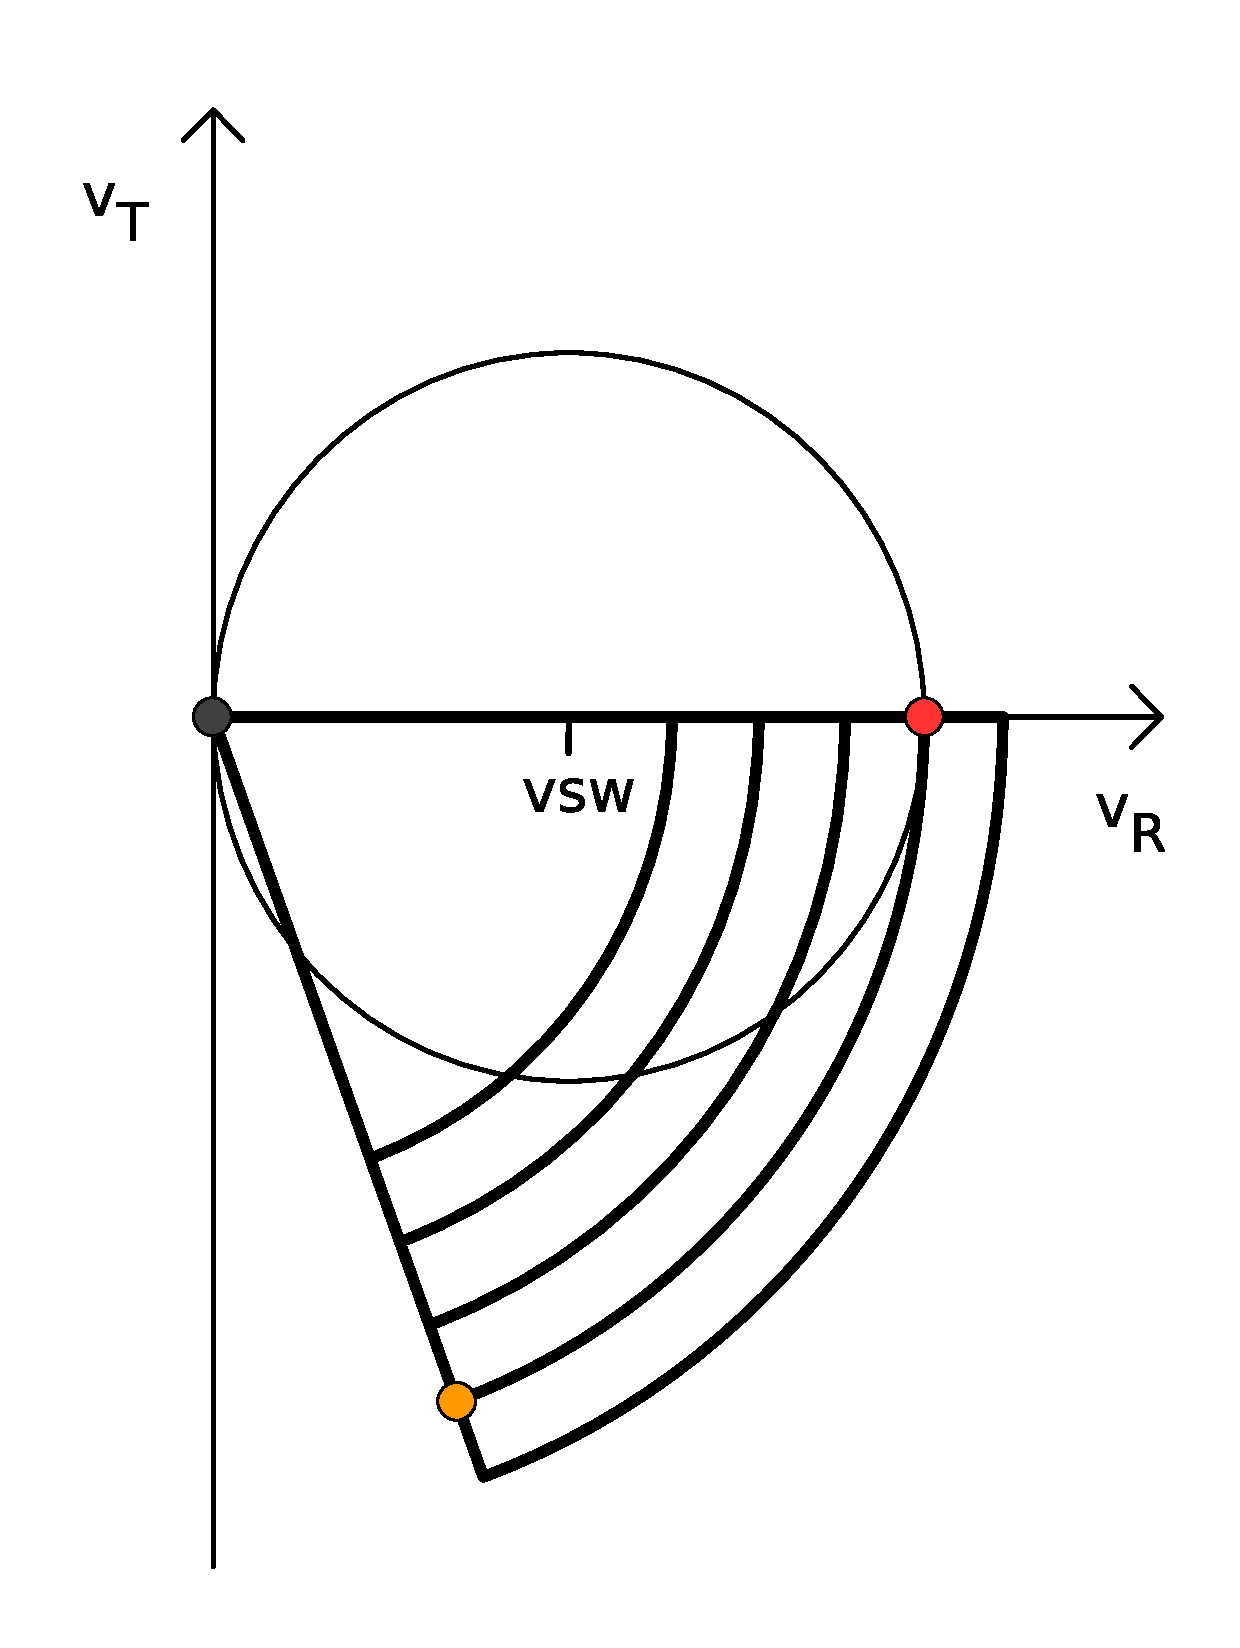
\includegraphics[scale=0.22]{Pics/swics_collimator111.pdf}}
		\only<2>{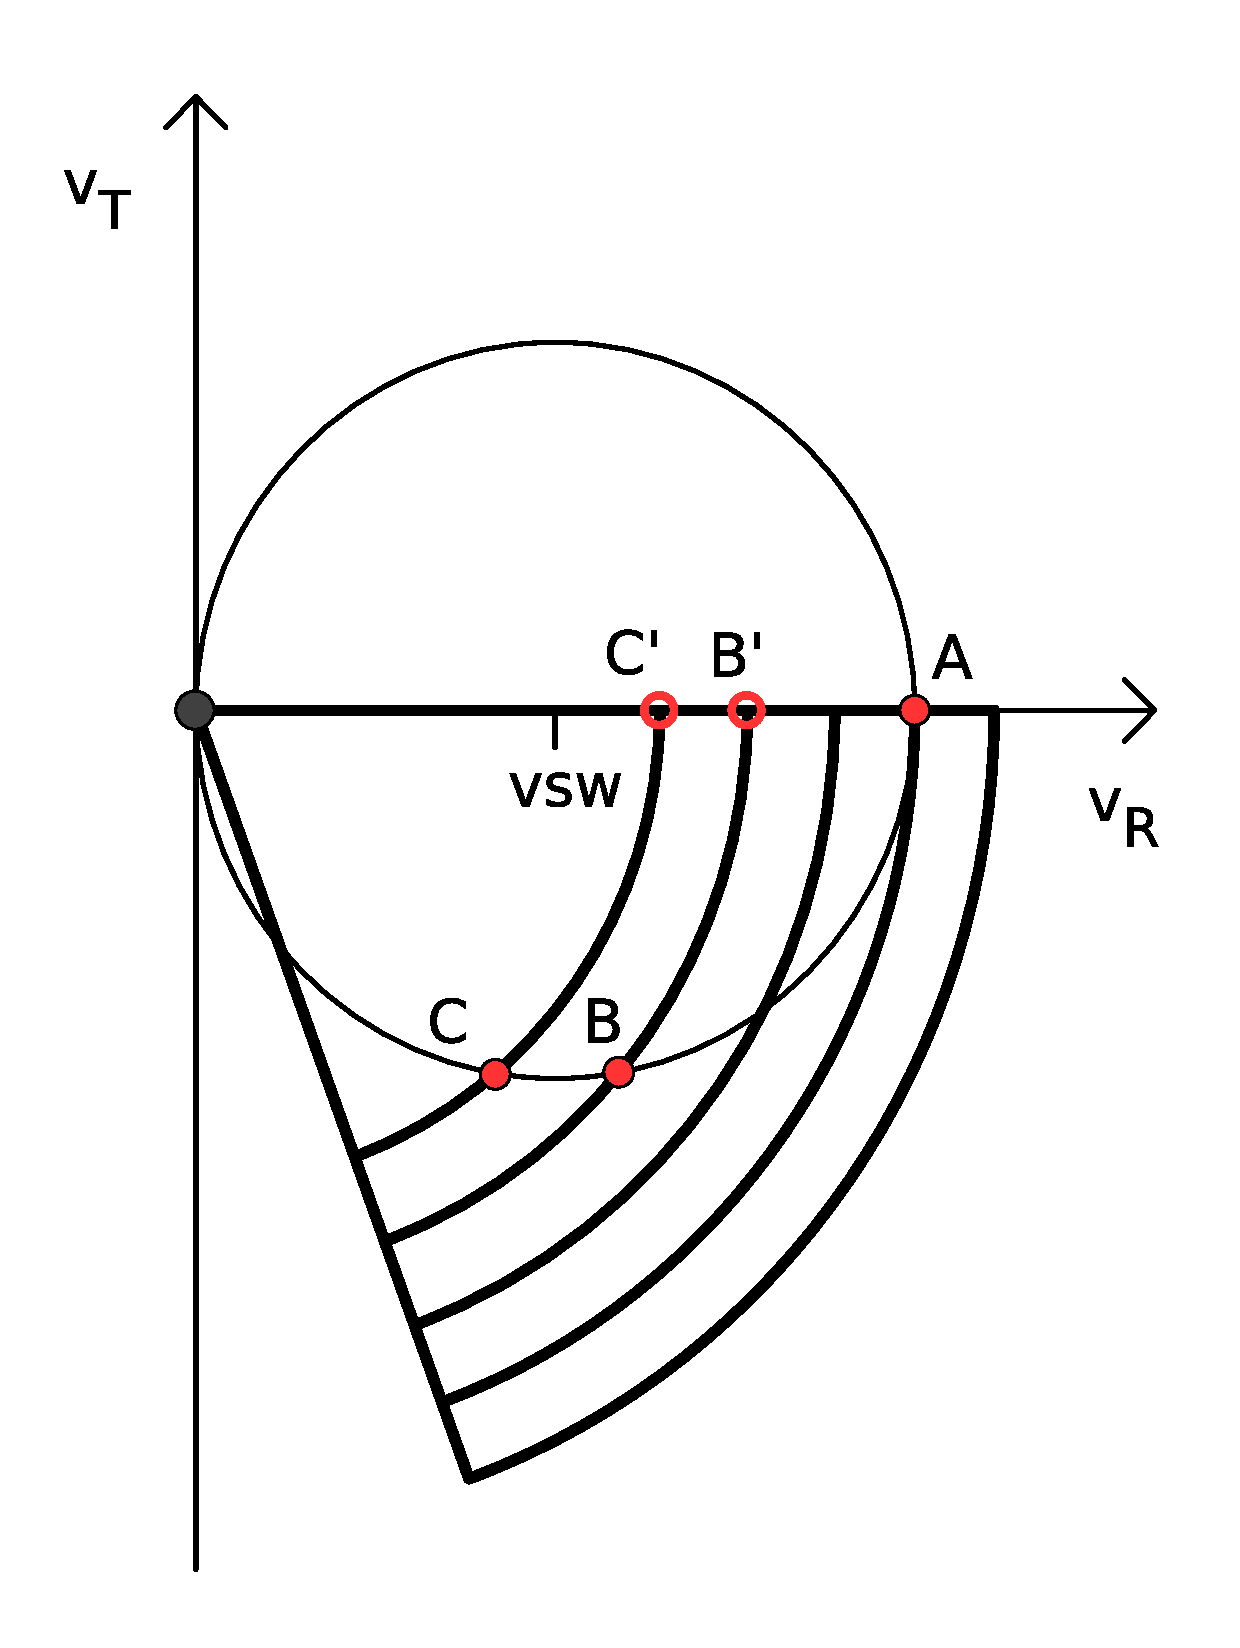
\includegraphics[scale=0.22]{Pics/swics_collimator22.pdf}}
	\end{columns}
\vspace{-0.1cm}
	\begin{itemize}
		\item For constant $\frac{m}{q}:$ $\frac{E}{q}$-step $\widehat{=}$ absolute value of velocity
		\only<2>{\item Integration over EpQ shells $\rightarrow$ loss of information!}
	\end{itemize}
\end{frame}
%%%
\begin{frame}{Angular resolution}
	\vspace{-.1cm}
	\begin{columns}
		\column{4.5cm}
		\begin{figure}									
			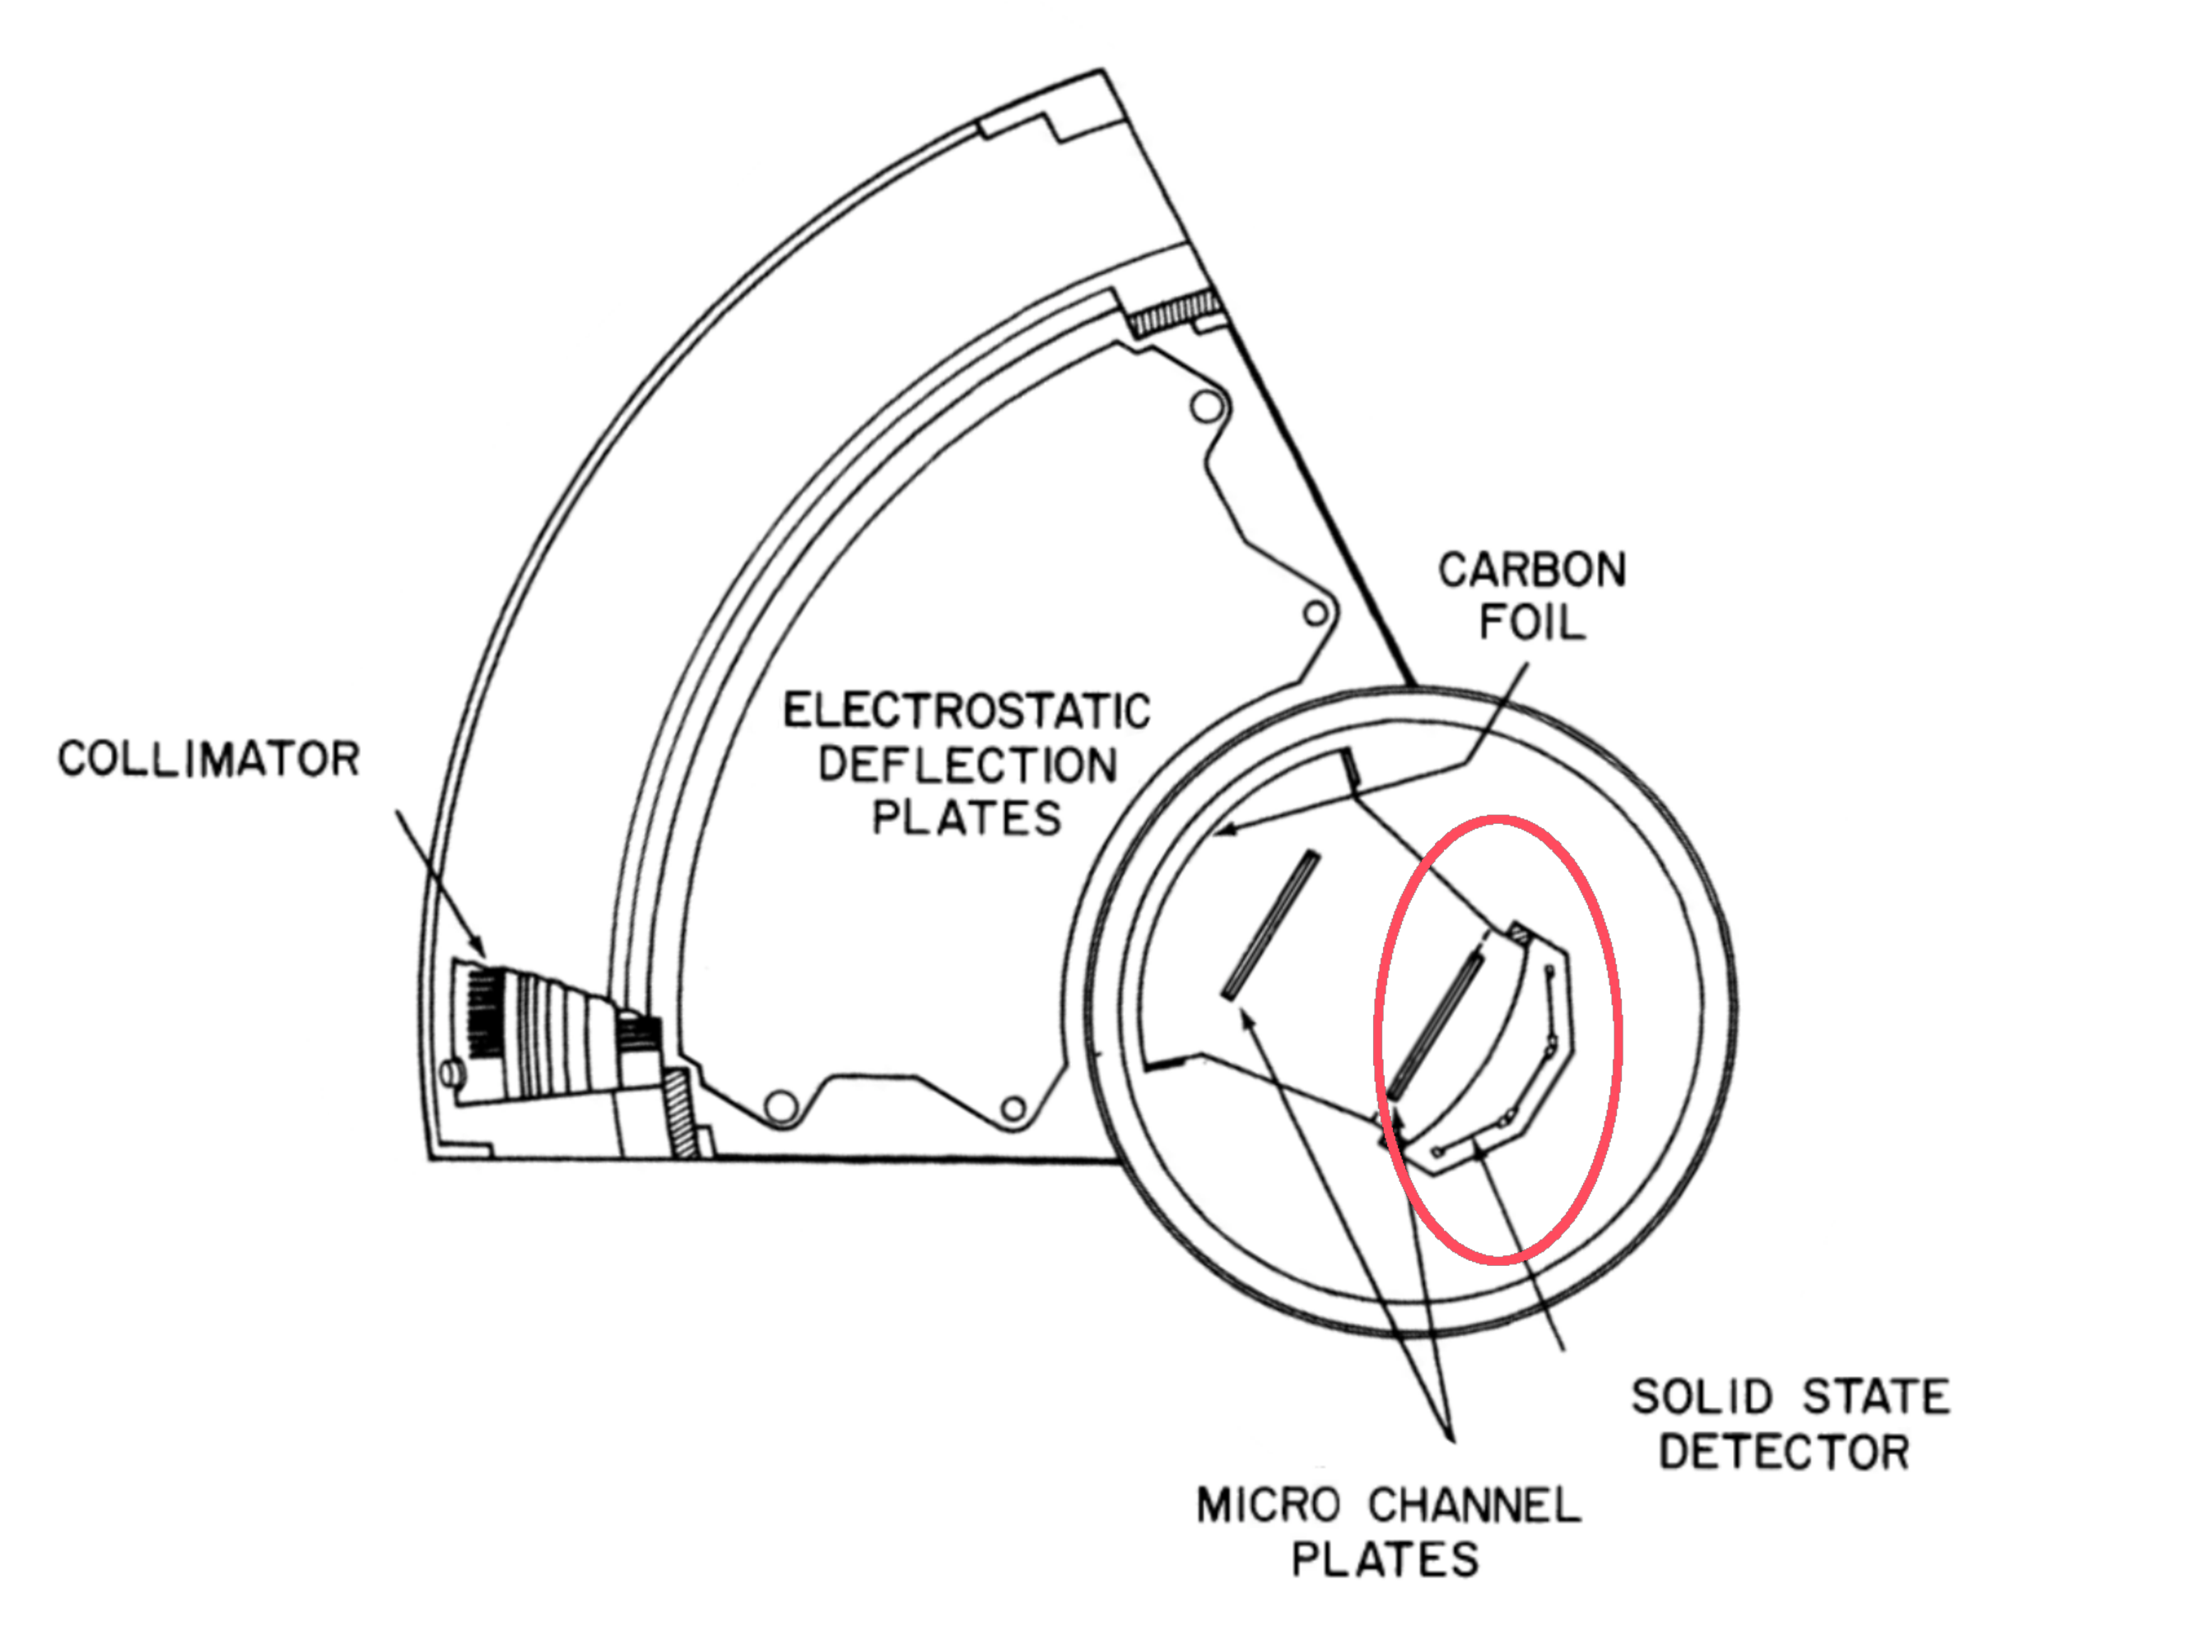
\includegraphics[scale=0.14]{Pics/swics_sensor_flipped_rotated_ellipse.pdf}
			
		\end{figure}
		\column{4cm}
		%\vspace{1.1cm}
		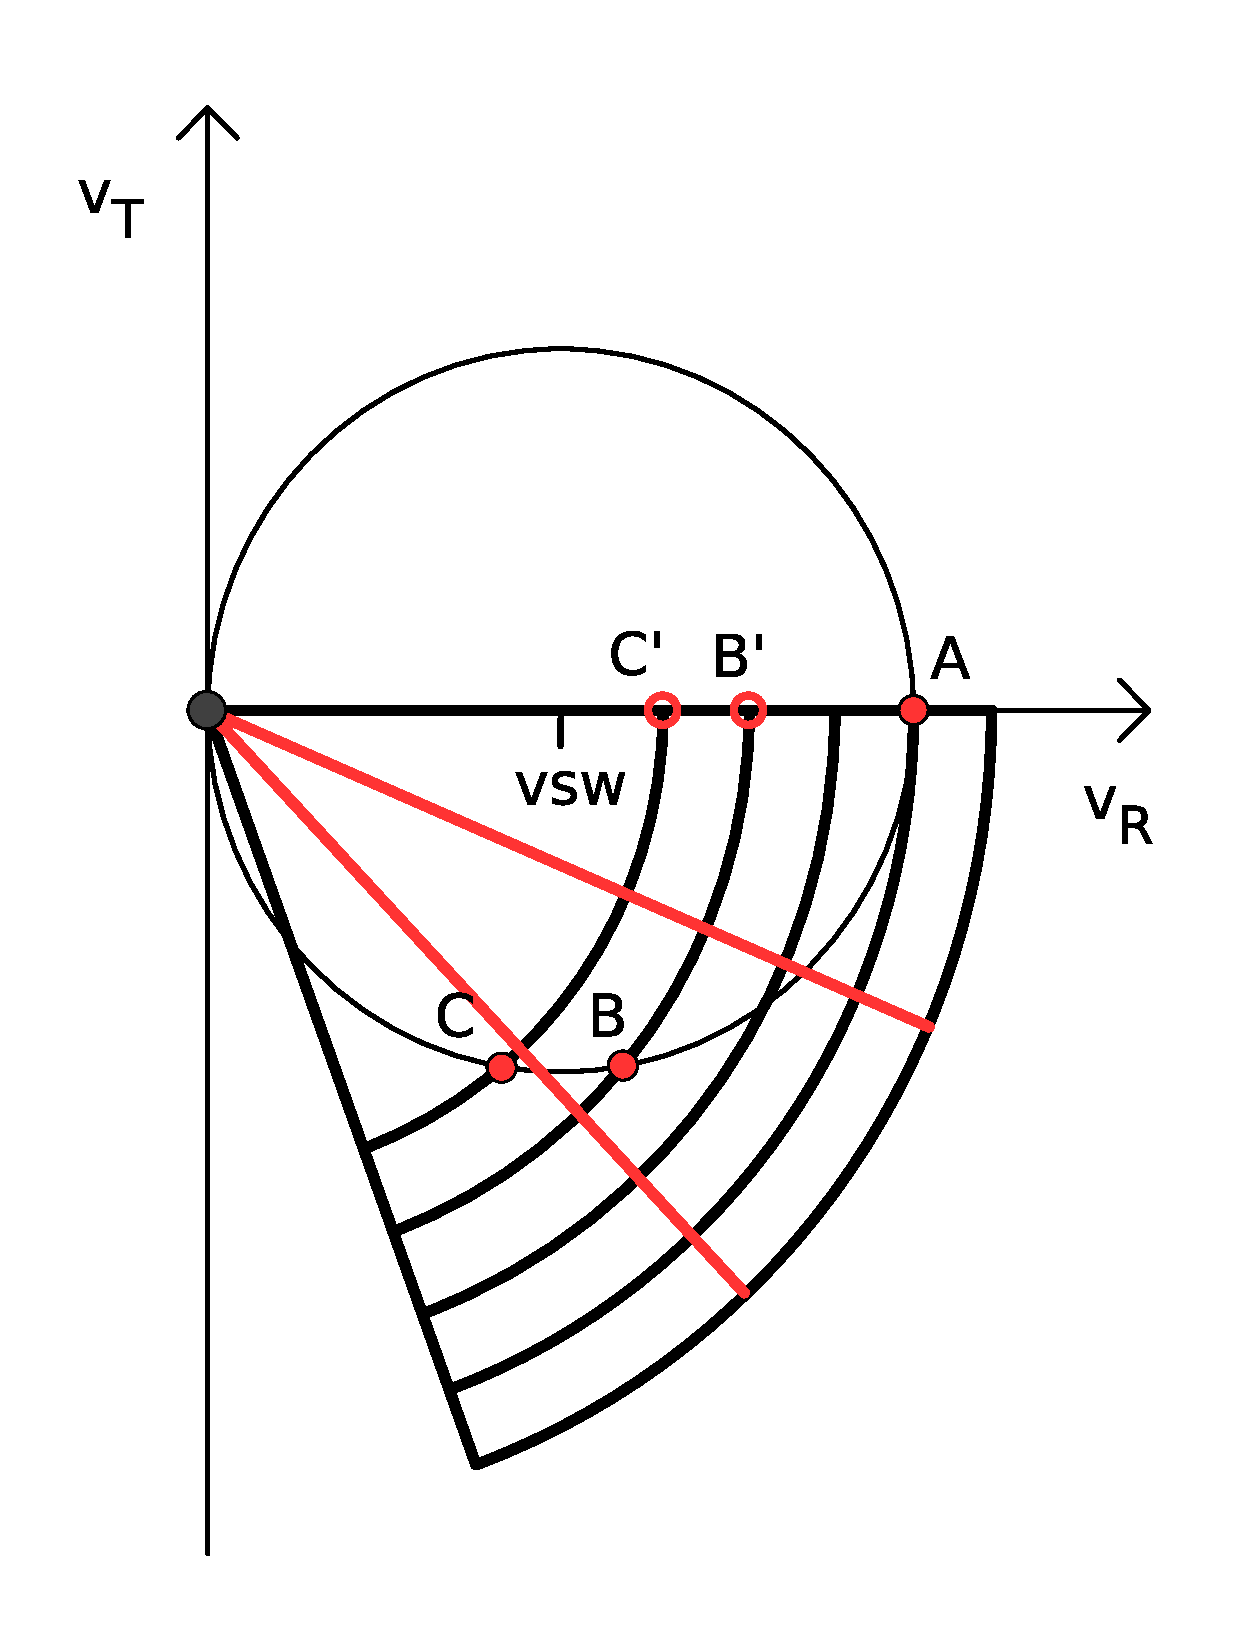
\includegraphics[scale=0.22]{Pics/swics_collimator33.pdf}
	\end{columns}
	\begin{itemize}
	\item SWICS: \textbf{3 detectors} \\ \small{Rough distinction between angles of incidence}
	\item \normalsize{3rd dimension: spin of the SC} \\ \small{Divided into \textbf{8 sectors}}
\end{itemize}
\end{frame}



%%%
\begin{frame}{The Virtual Detector}
	\begin{columns}
		\column[]{6.5cm}
		\begin{figure}
					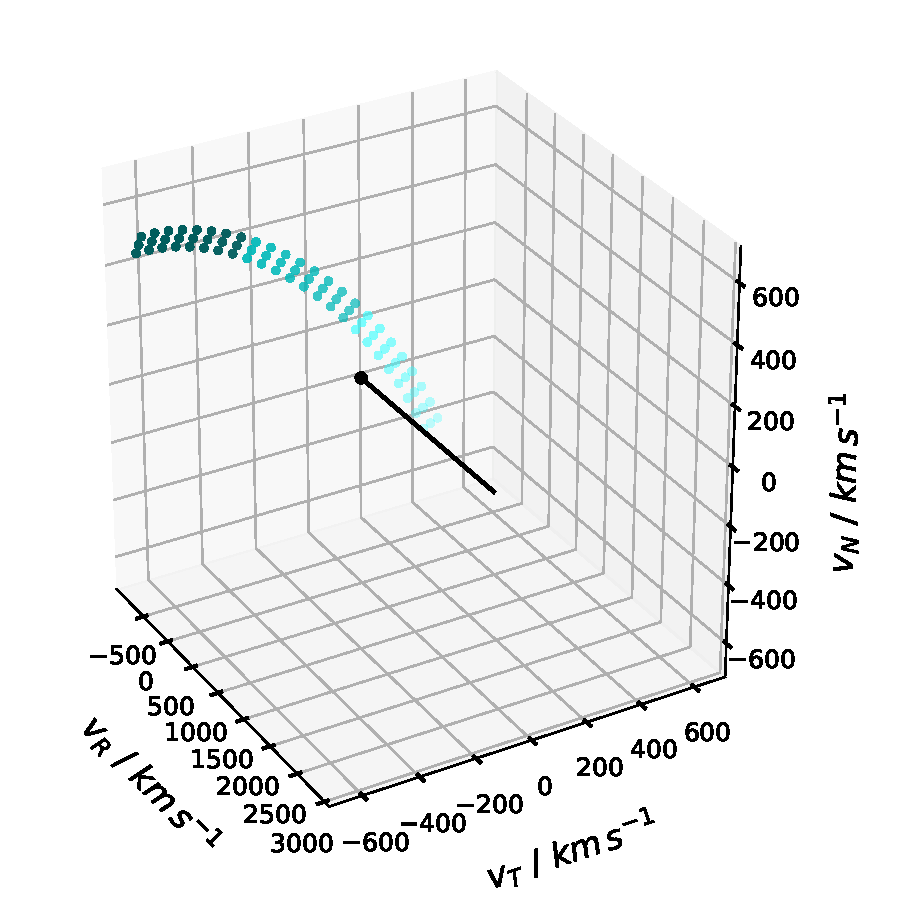
\includegraphics[scale=0.35]{Pics/col_single_new.pdf}
			\end{figure}
	{\scriptsize \begin{center}
				Unrotated collimator acceptance \\ for one EpQ step
	\end{center}}

		\column[]{6.5cm}
				\begin{figure}
			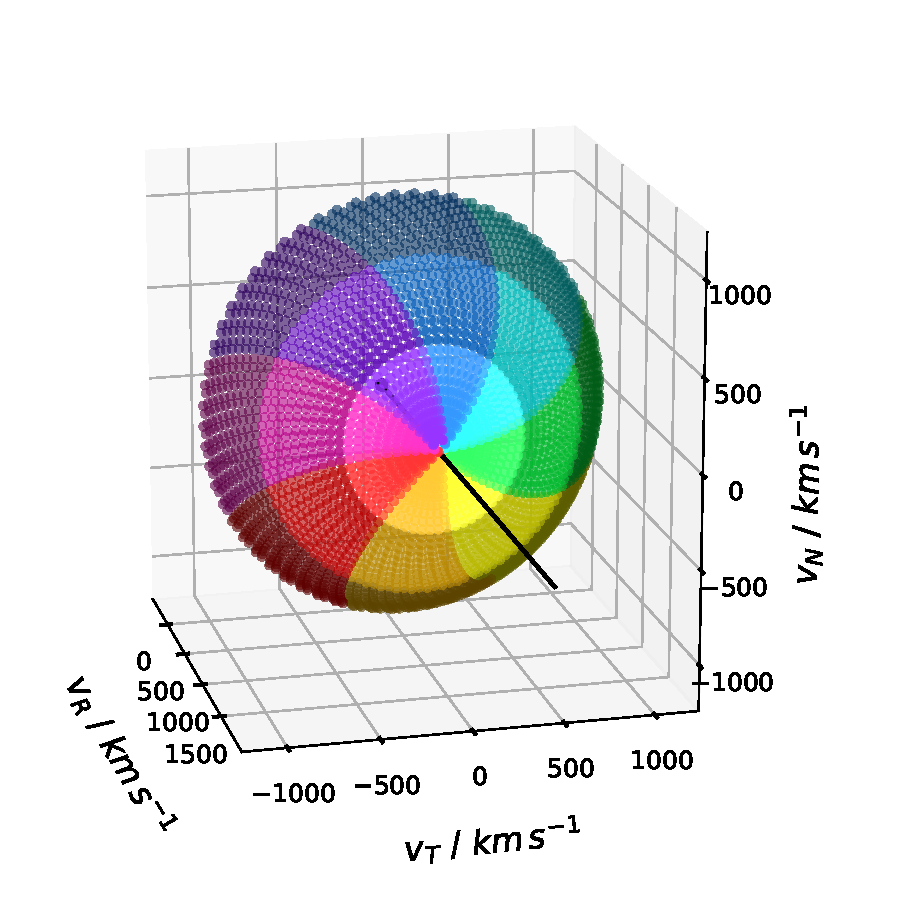
\includegraphics[scale=0.38]{Pics/col_vspace_normal.pdf}
		\end{figure}
		\begin{center}
			{\scriptsize Collimator Acceptance for \\one spacecraft spin and one EpQ step}
		\end{center}
	\end{columns}
	
\end{frame}
%%%

%%%
\section{Methods -- The Virtual Detector}
\begin{frame}{The Virtual Detector}
\begin{columns}
	\column[]{6.5cm}
	\begin{figure}
	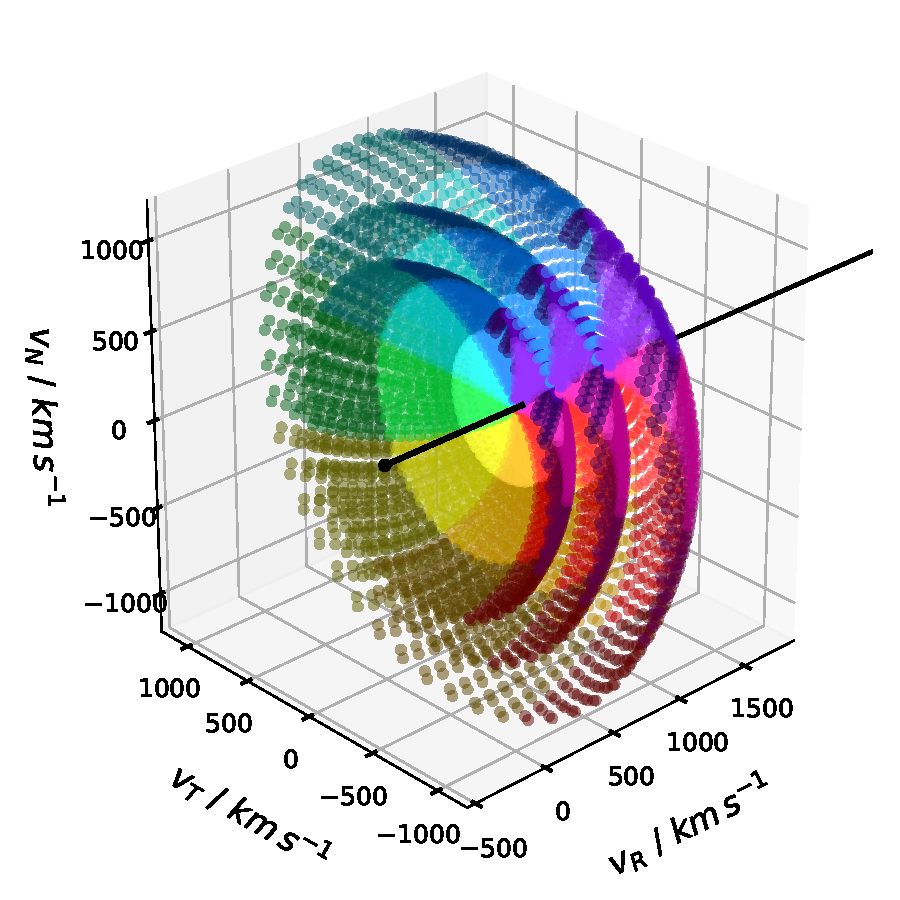
\includegraphics[scale=0.35]{Pics/col_shells.pdf}
\end{figure}
	
	
	\column[]{6.5cm}
	\begin{figure}
		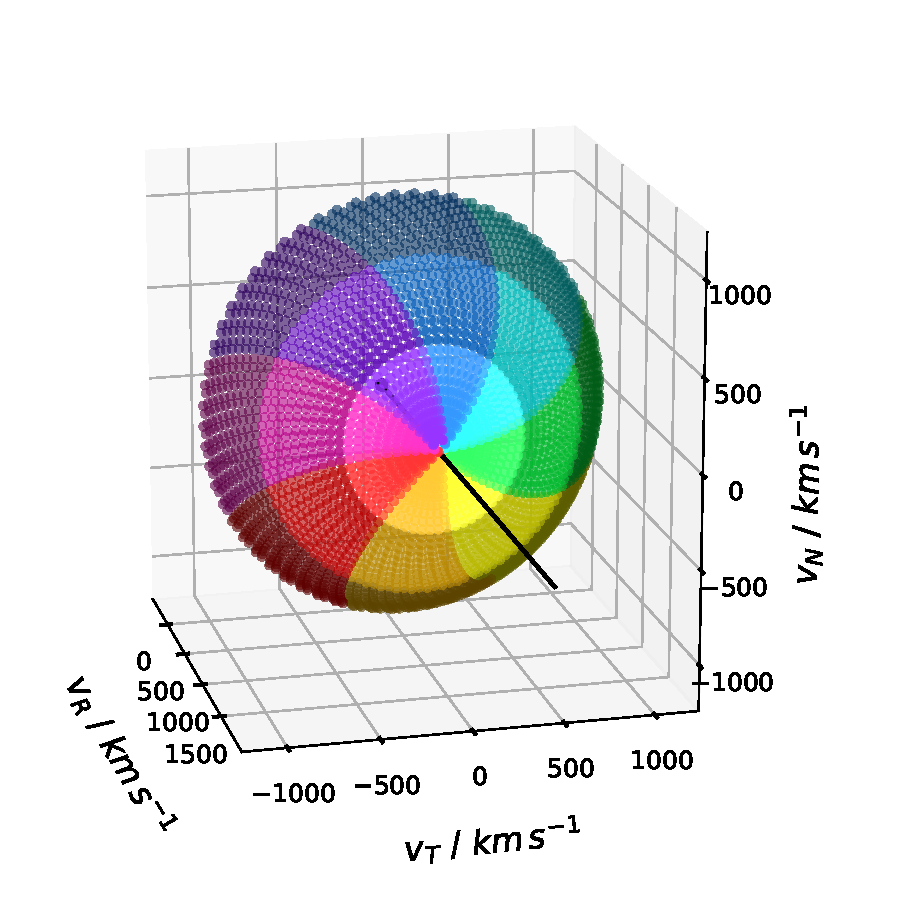
\includegraphics[scale=0.38]{Pics/col_vspace_normal.pdf}
	\end{figure}

\end{columns}

\end{frame}


%%%



%%%

\begin{frame}{Aspect Angle}
\begin{figure}
	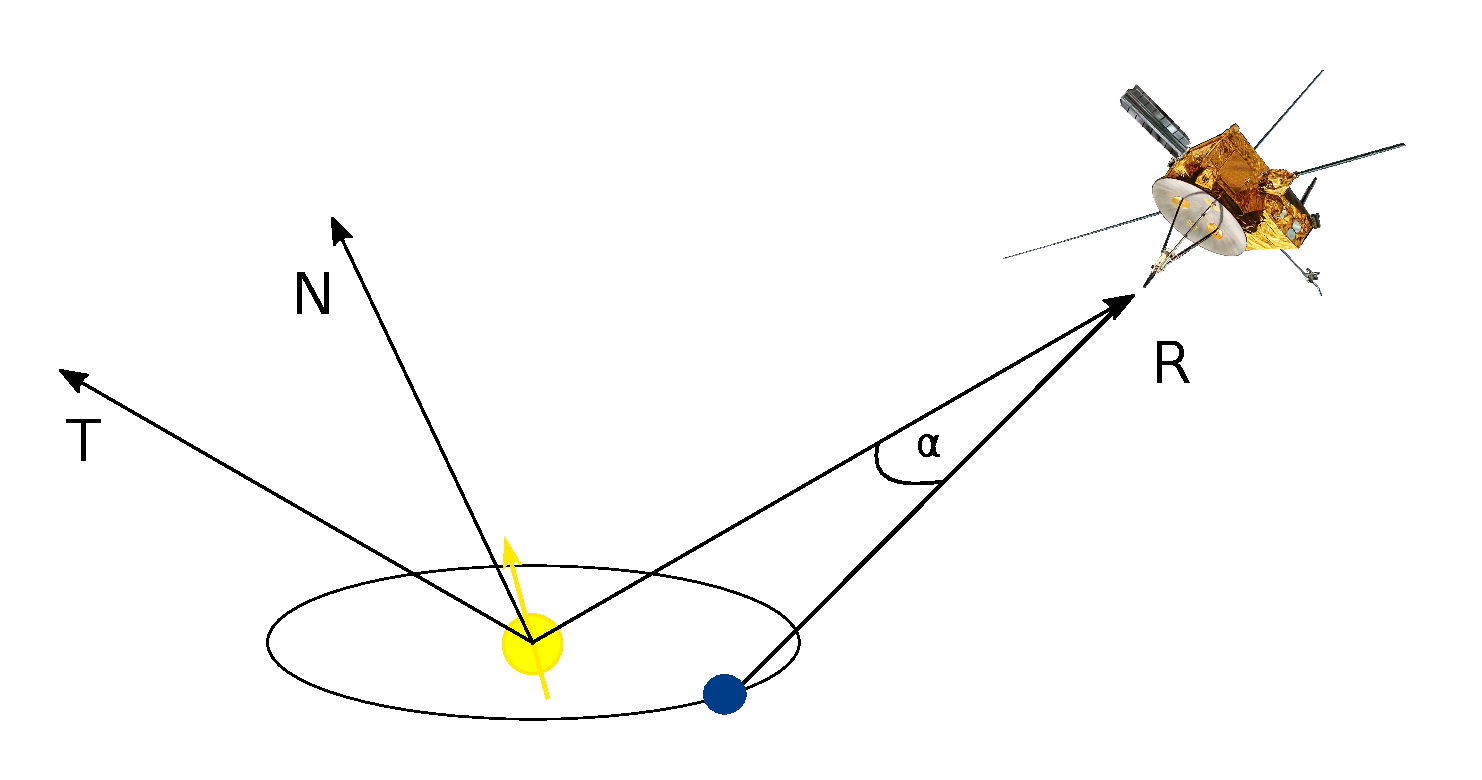
\includegraphics[scale=0.45]{Pics/RTN_AA_flat_angle.pdf}
\end{figure}
\end{frame}

%%%

\begin{frame}{Aspect Angle}
\begin{figure}
	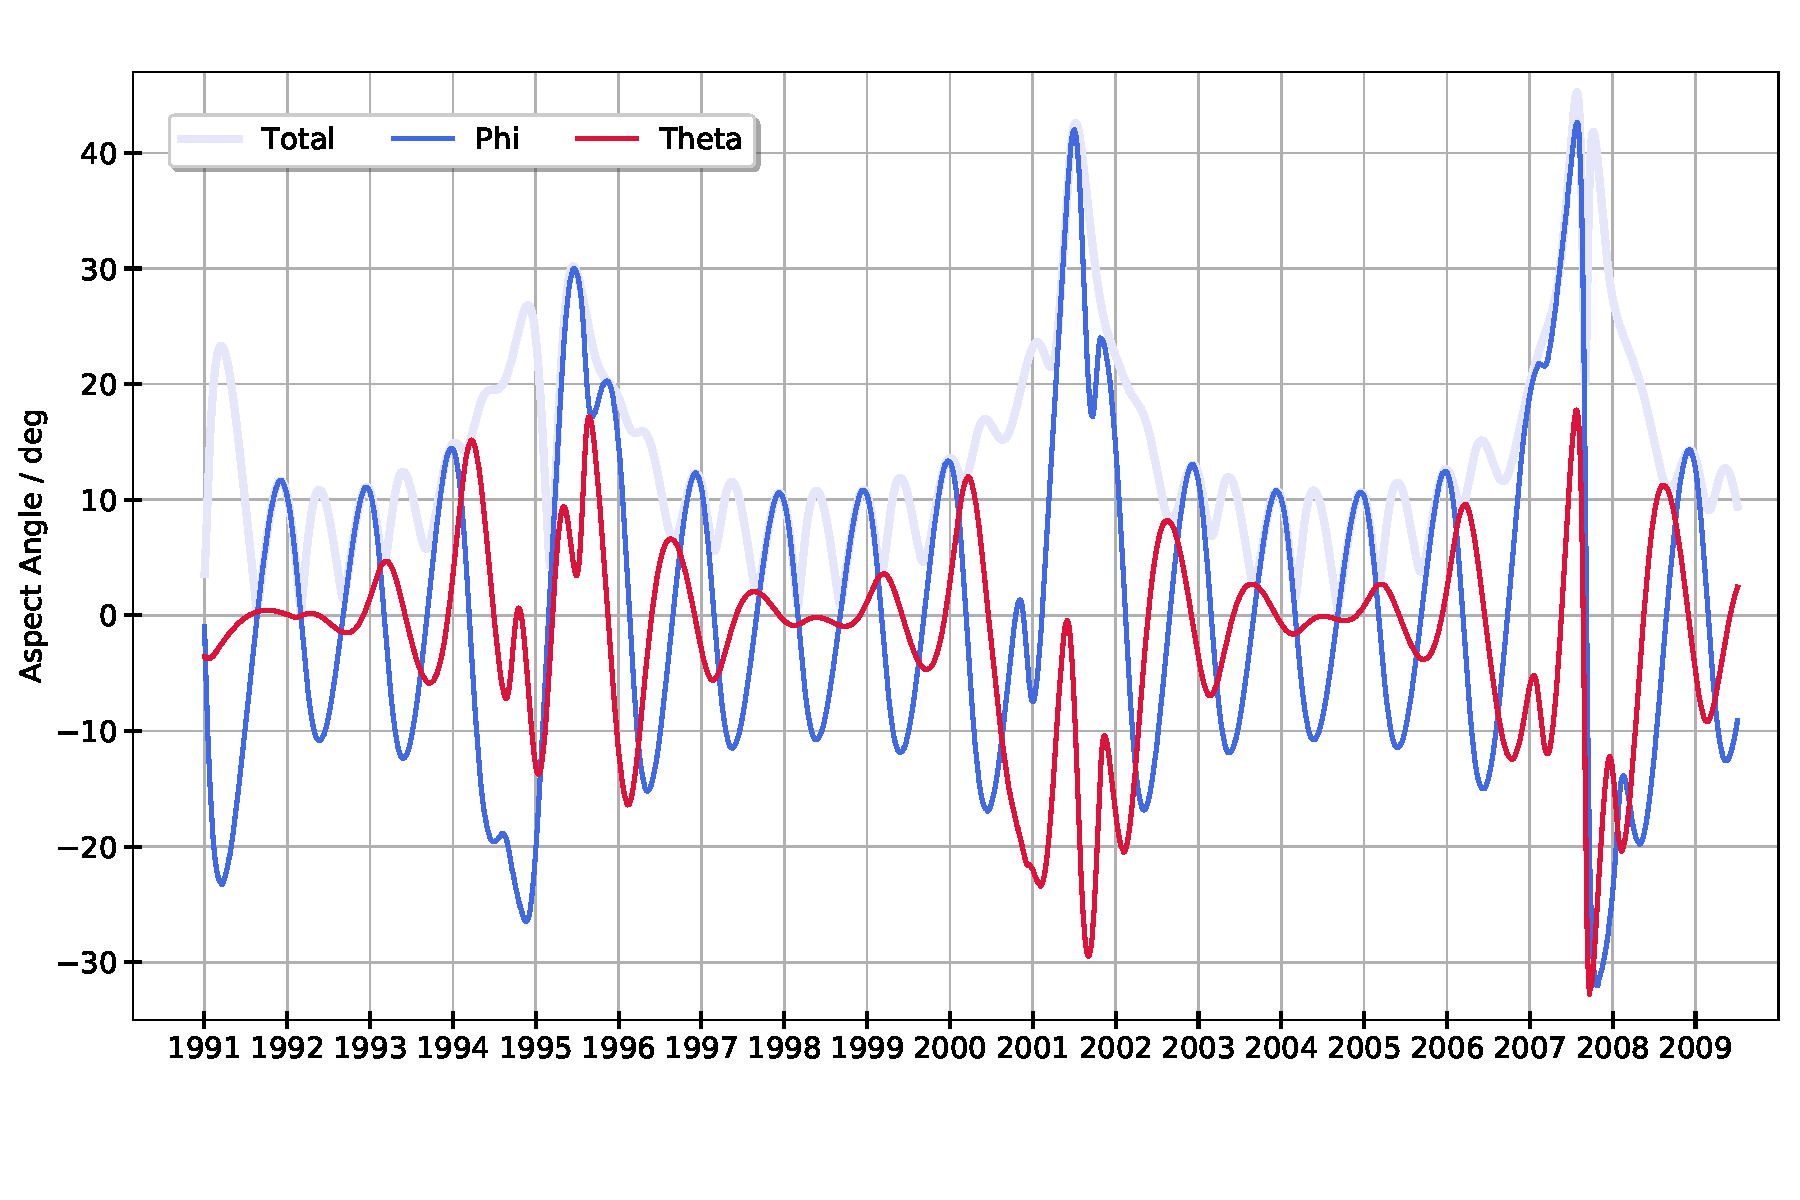
\includegraphics[scale=0.37]{Pics/aa_new.pdf}
\end{figure}
\end{frame}

%%%

\begin{frame}{Aspect Angle}
\begin{columns}
	\column[]{6.cm}
	\vspace{-0.8cm}
		\begin{figure}
			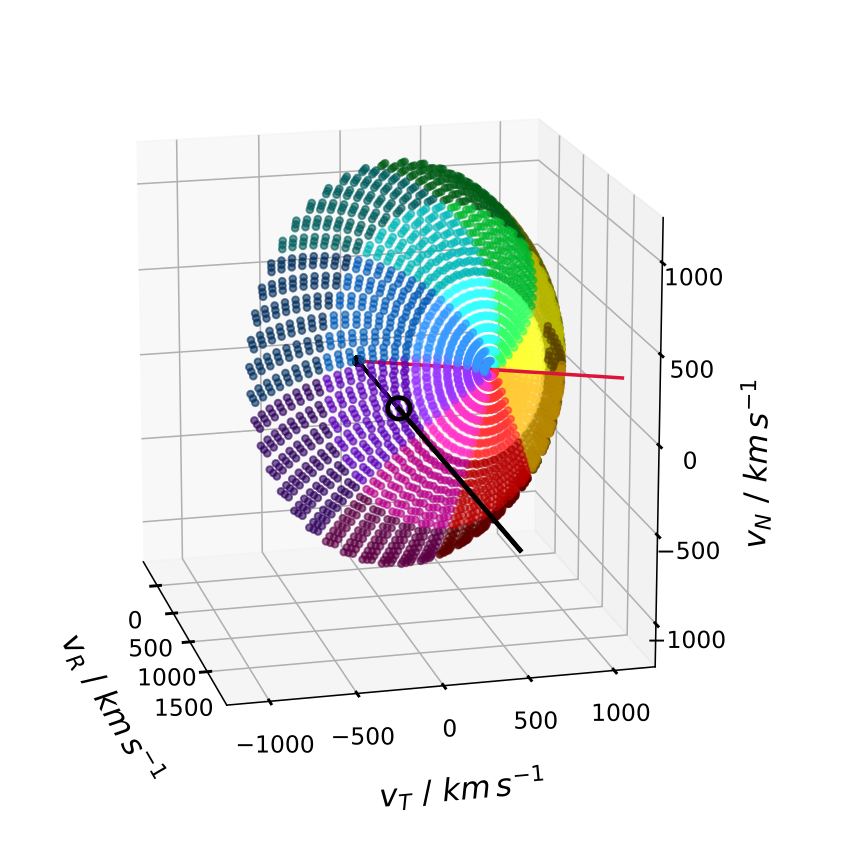
\includegraphics[scale=0.4]{Pics/col_aa_marker.png}
		\end{figure}
\begin{center}
	{\small 	Aspect angle:\\
	$\varphi = 25 ^\circ, \vartheta = -10 ^\circ $}
\end{center}
	
	\column[]{6cm}
	
		\begin{figure}
			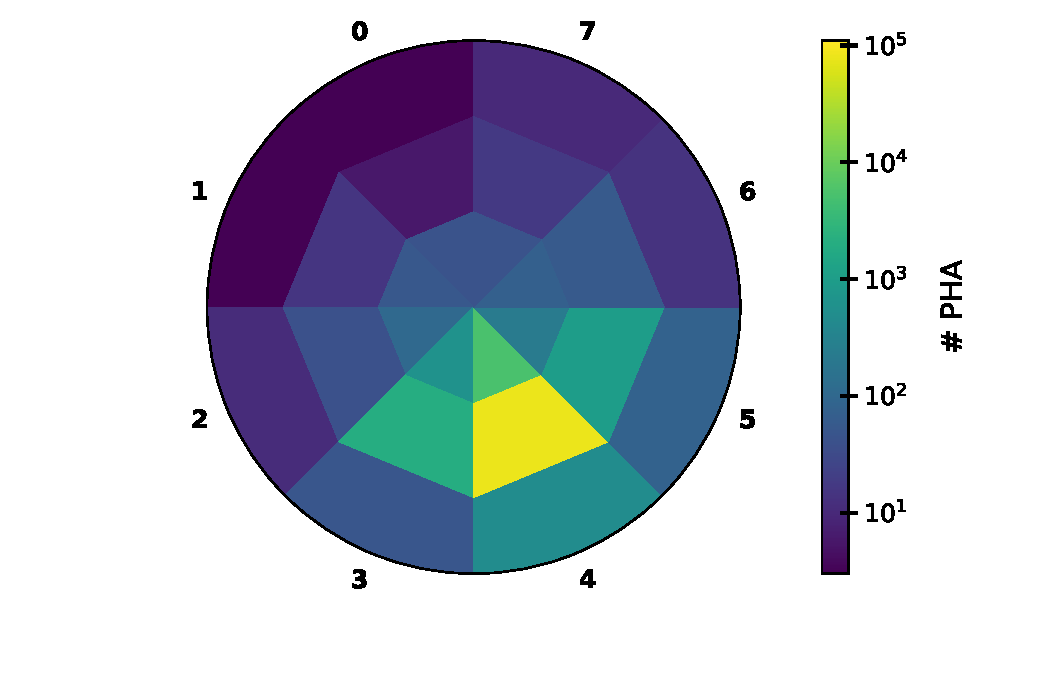
\includegraphics[scale=0.4]{Pics/hist_det_sec_aa_90days2001.pdf}
		\end{figure}
\begin{center}
		
{\small 	$\Rightarrow$ Plausibility check with \\solar wind $\mathrm{He^{2+}}$ PHA data}\\{\scriptsize  ( 120 days in 2001)}
\end{center}
	\column[]{1cm}
\end{columns}


\end{frame}

%%%

\begin{frame}{Frame of Reference}
\begin{columns}
\column[]{5cm}
\vspace{-1cm}
	\begin{figure}
		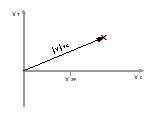
\includegraphics[scale=2.2]{Pics/vspace_sc_trans.pdf}
	\end{figure}
	\vspace{-1.2cm}
	\begin{figure}
	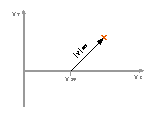
\includegraphics[scale=2.2]{Pics/vspace_sw_trans.pdf}
\end{figure}


\column[]{6.2cm}
	\vspace{.5cm}
	\begin{figure}
		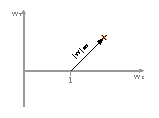
\includegraphics[scale=2.2]{Pics/wspace_sw_trans.pdf}
	\end{figure}
\end{columns}
\end{frame}

%%%

%%%
\section{Results -- 3D VDF}
\begin{frame}{Spherical Cut through VDF}
\begin{columns}
	\column{2.5cm}
\begin{figure}
	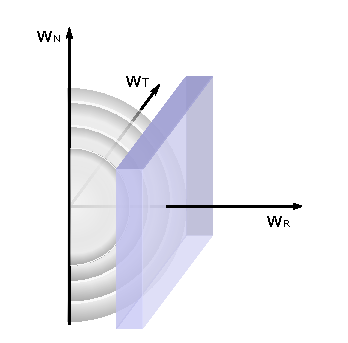
\includegraphics[scale=.7]{Pics/slice_R2.pdf}
\end{figure}
{\scriptsize 50 days in 1993 \\
 $\mathrm{vsw} : 760 - 780 \, \mathrm{km\,s^{-1}}$
}
\column{7.5cm}
\begin{figure}
	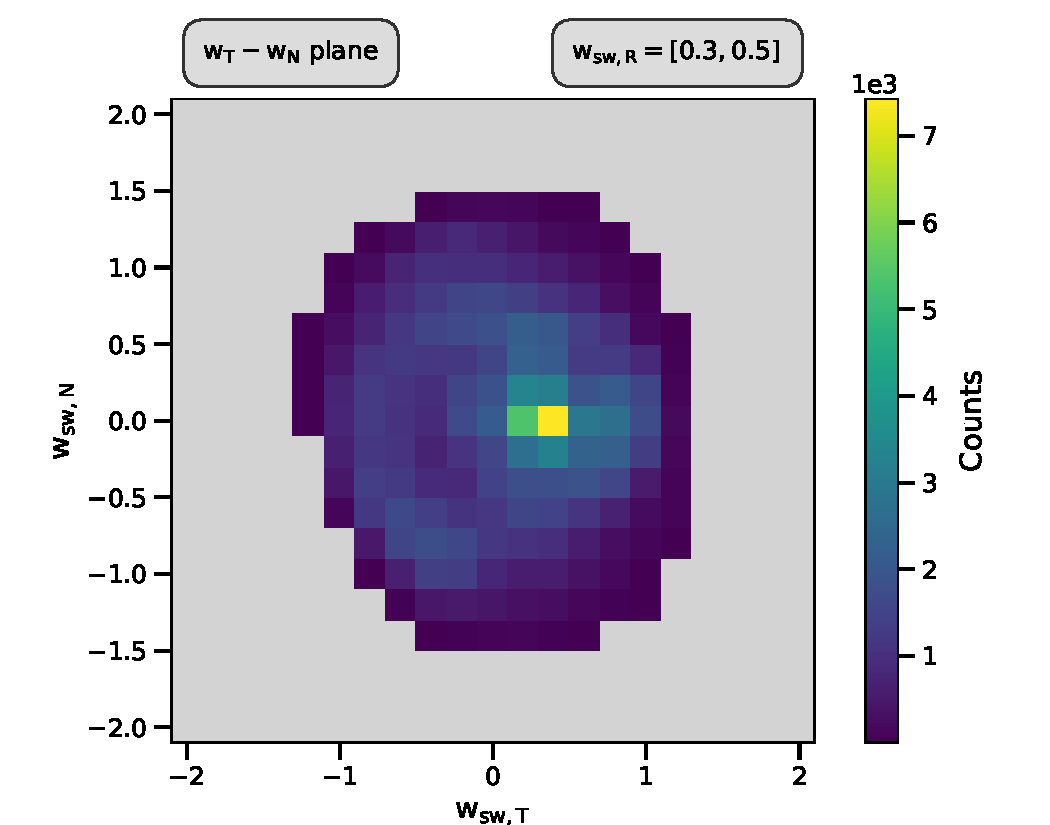
\includegraphics[scale=.5]{Pics/cart_50_counts_R.pdf}
\end{figure}
\end{columns}
\end{frame}

%%%


%%%

\begin{frame}{From Counts to Phase Space Density}
\begin{columns}
	\column[]{2cm}
	\begin{mdframed}[roundcorner=4pt,userdefinedwidth=3.cm,
		align
		=center,
		linecolor
		=black,backgroundcolor=blue!8,
		linewidth
		=1.pt]
		$PSD = \frac{N}{PSV}$
	\end{mdframed}

	\column[]{6cm}
	
	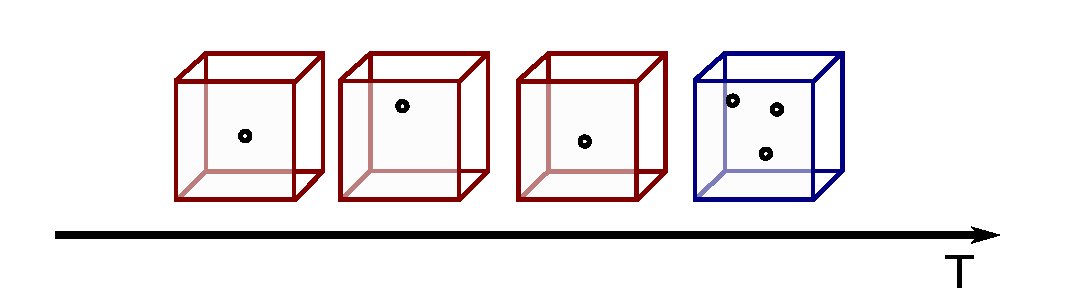
\includegraphics[scale=.4]{Pics/norm_time.pdf}
\end{columns}


\begin{columns}
	\column[]{5.5cm}
	\begin{figure}
		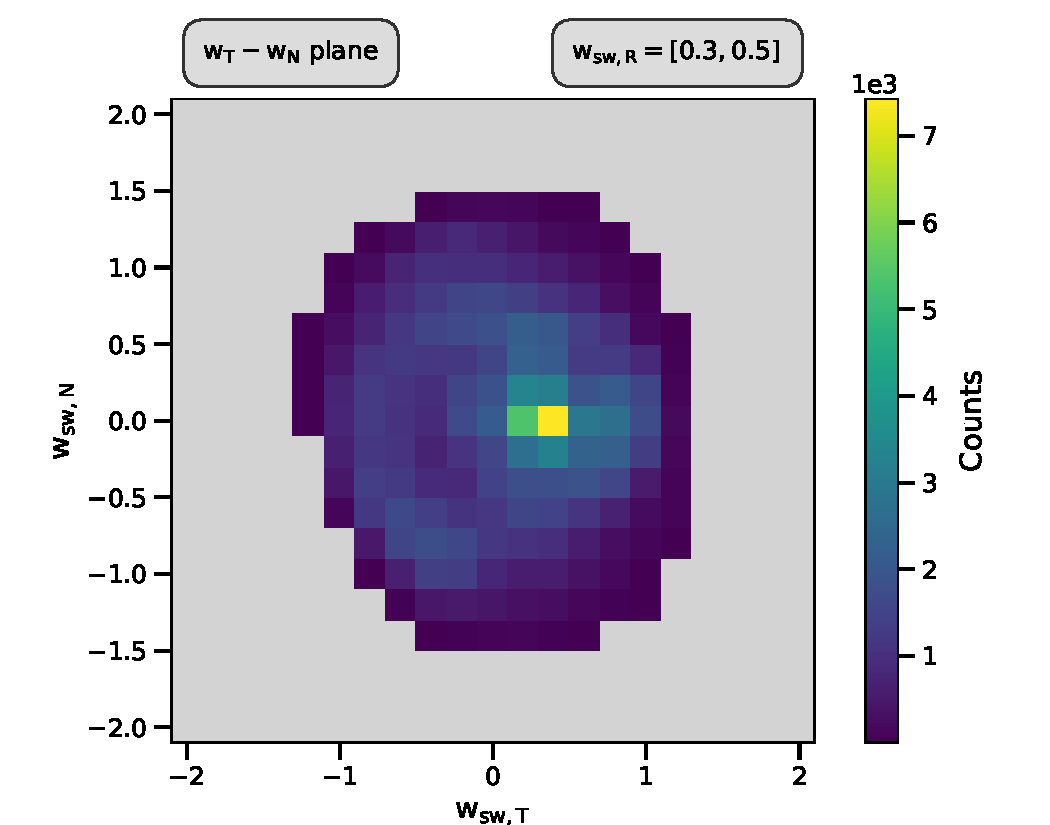
\includegraphics[scale=.35]{Pics/cart_50_counts_R.pdf}
	\end{figure}
	\column[]{5cm}
	\begin{figure}
		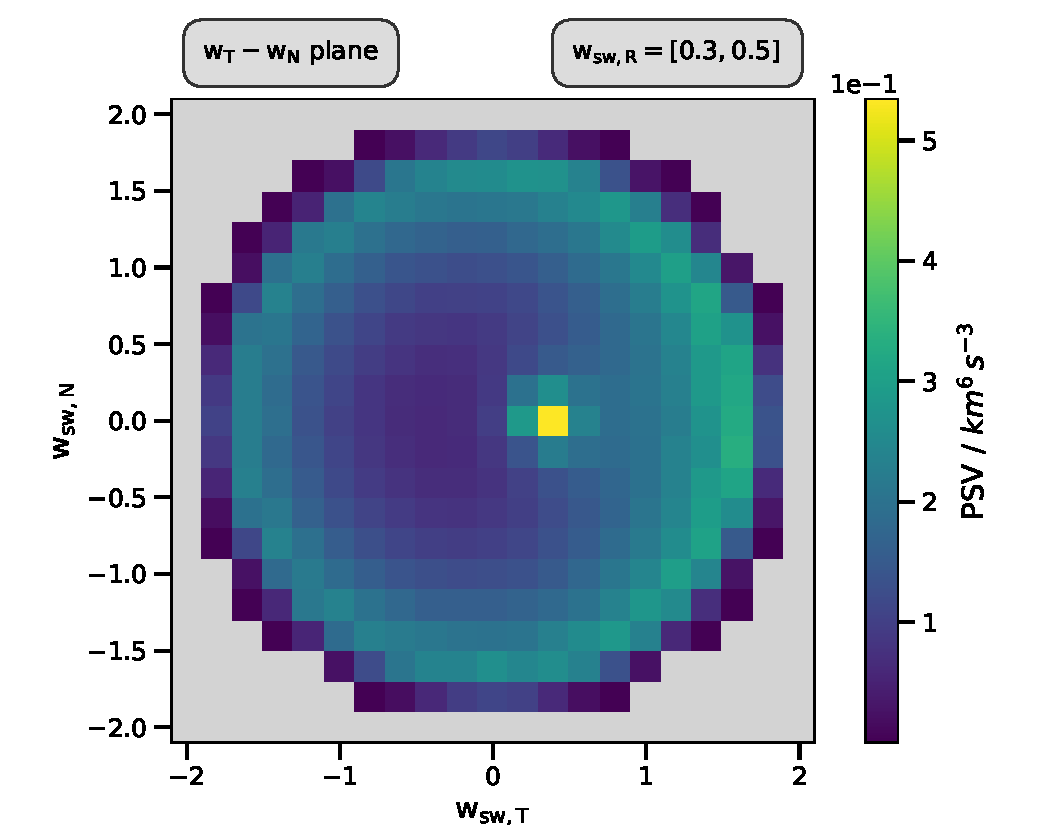
\includegraphics[scale=.35]{Pics/cart_50_norm_R.pdf}
	\end{figure}
\column[]{1cm}
	\end{columns}

\end{frame}

%%%

\begin{frame}{Spherical Cut through VDF}
\begin{columns}
	\column{3cm}
	\begin{figure}
		
		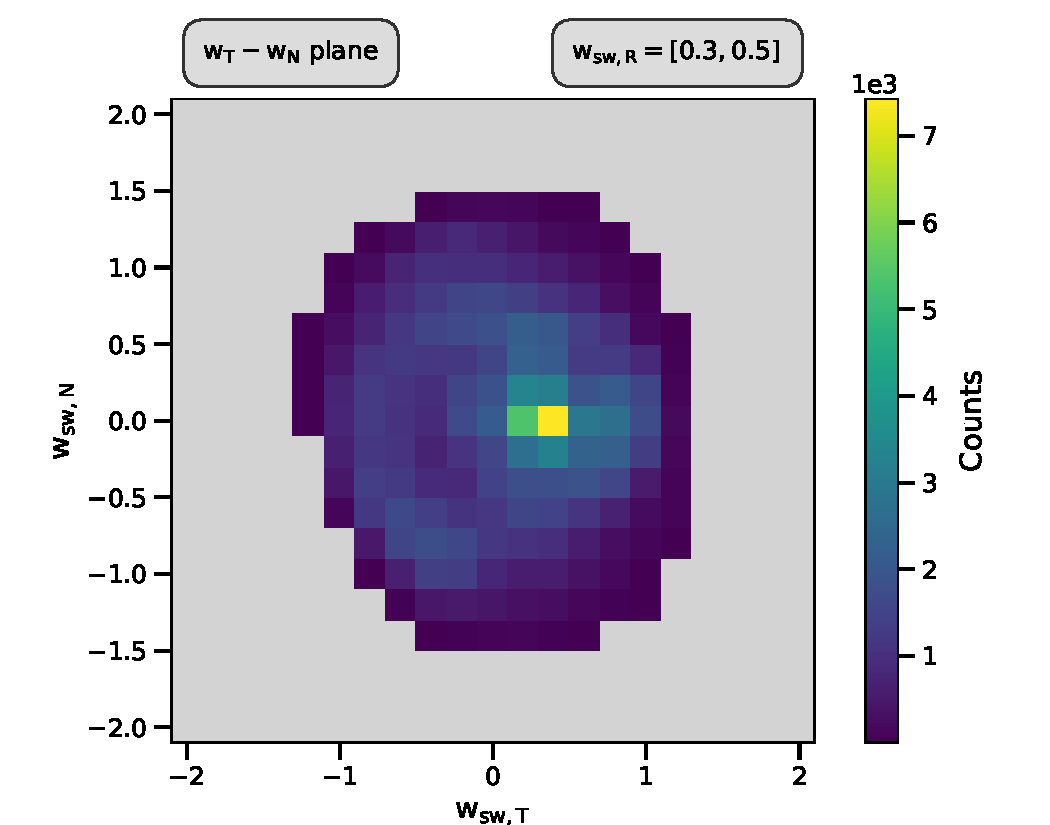
\includegraphics[scale=.2]{Pics/cart_50_counts_R.pdf}
		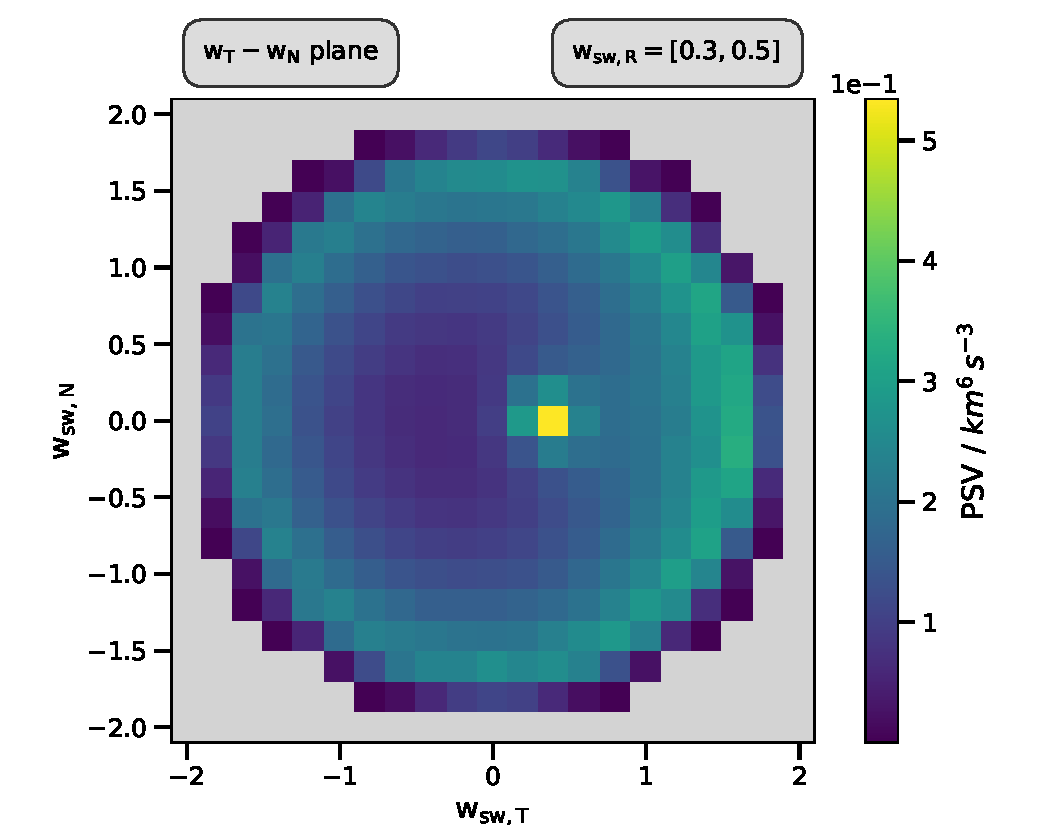
\includegraphics[scale=.2]{Pics/cart_50_norm_R.pdf}
		
	\end{figure}
	\column{6.5cm}
	\begin{figure}
	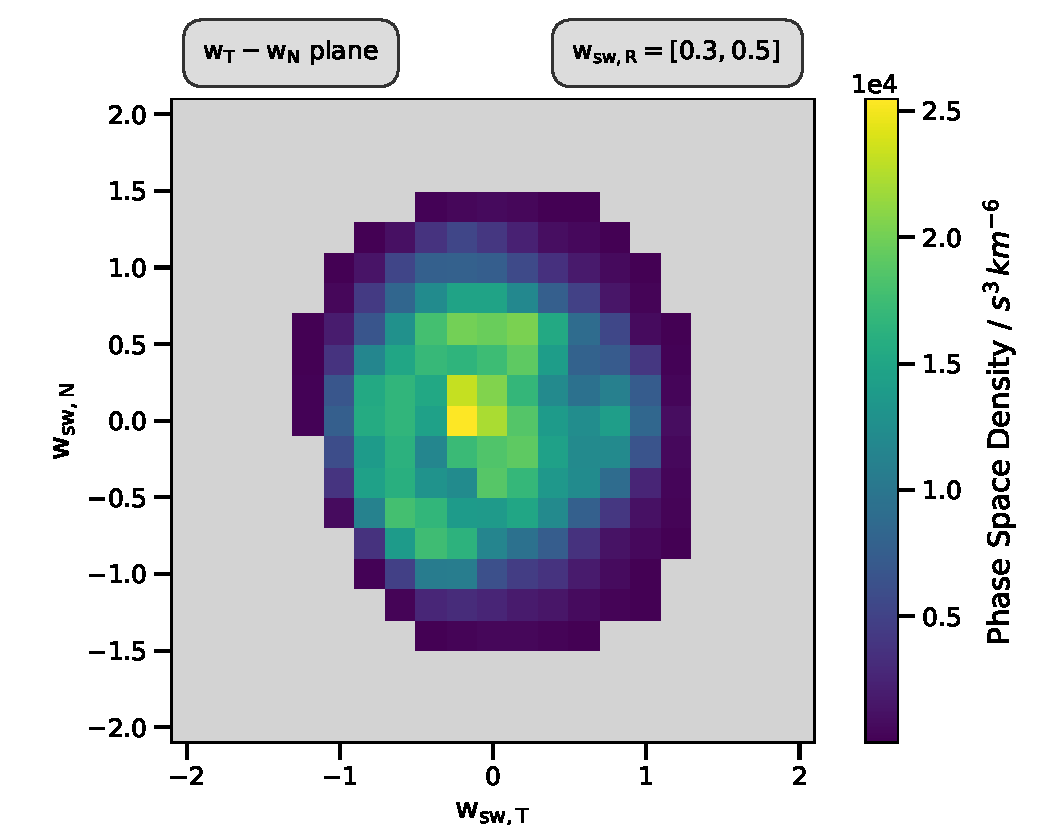
\includegraphics[scale=.45]{Pics/cart_50_ps_R.pdf}
	\end{figure}
\column{.5cm}
\end{columns}
\end{frame}



%%%
\begin{frame}{Spherical Surface}
\begin{columns}
	\column{5.5cm}
	\begin{figure}
		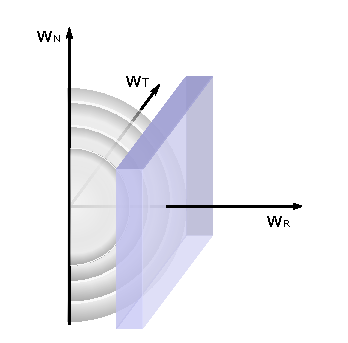
\includegraphics[scale=.8]{Pics/slice_R2.pdf}
	\end{figure}

	\column{7.5cm}
\begin{figure}
	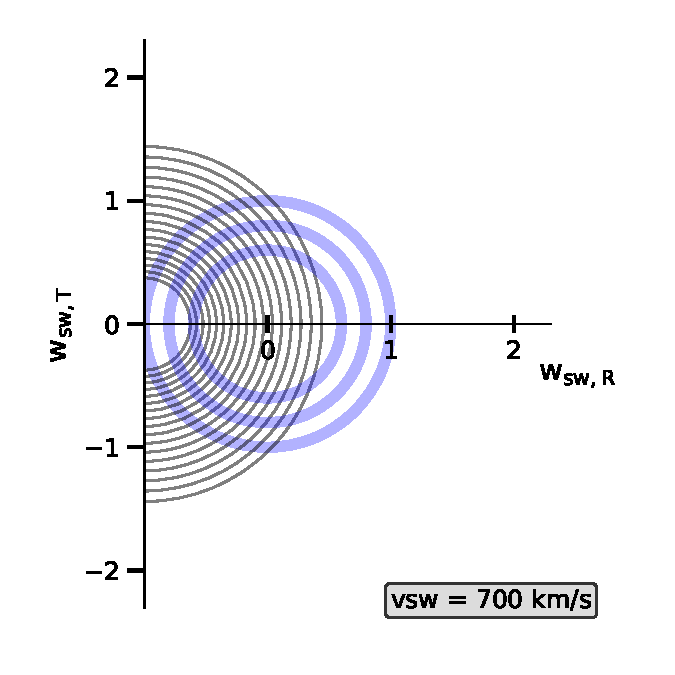
\includegraphics[scale=.65]{Pics/cov.pdf}
\end{figure}
\end{columns}
\end{frame}

%%%
\begin{frame}{Spherical Surface}
\begin{columns}
\column{1.8cm}
\vspace{-4.5cm}
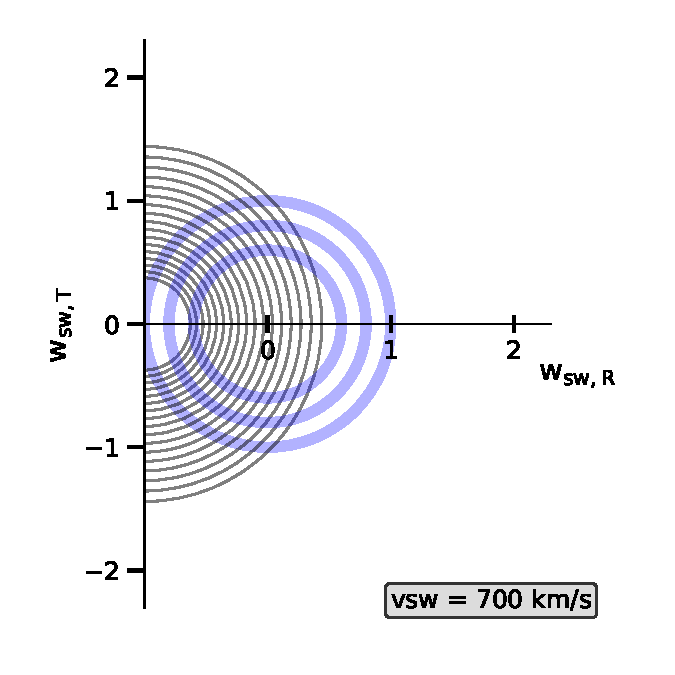
\includegraphics[scale=.3]{Pics/cov.pdf}

			
\column{16cm}
\vspace{2.2cm}

	
	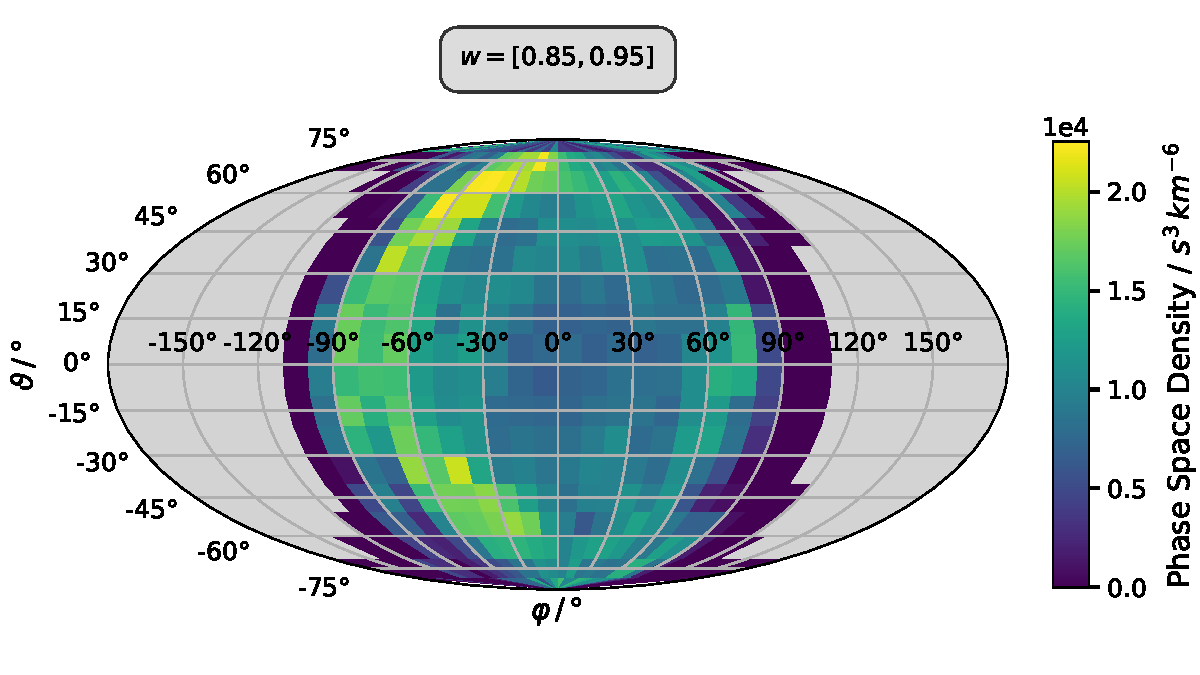
\includegraphics[scale=.51]{Pics/sky_ps.pdf}

\vspace{-0.9cm}
\begin{center}
	 {\tiny $\mathrm{vsw}:760 - 780 \, \mathrm{km\,s^{-1}}$ --
		50 days in 1993}
\end{center}
\column{4cm}
\end{columns}
\end{frame}




%%%

\begin{frame}{1D Spectrum}
\begin{columns}
		\column{.1cm}
	\column{4.8cm}

	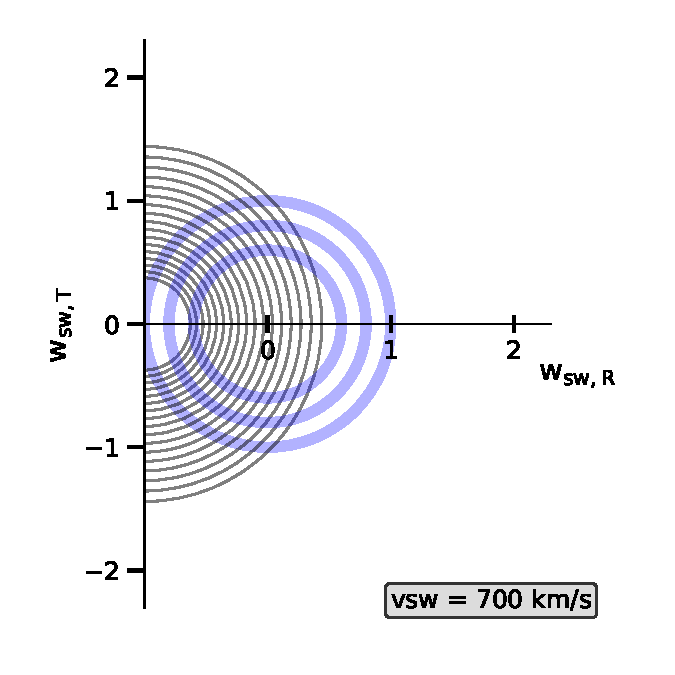
\includegraphics[scale=.3]{Pics/cov.pdf}
	\hspace{1cm}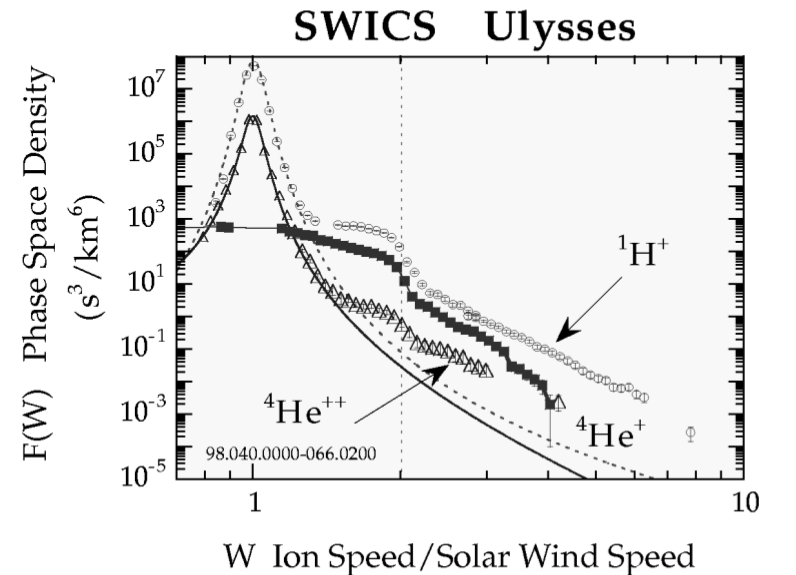
\includegraphics[scale=0.15]{Pics/sw_pui_gloeckler.png}
	
	\column{6cm}
	\vspace{.5cm}
	
	
	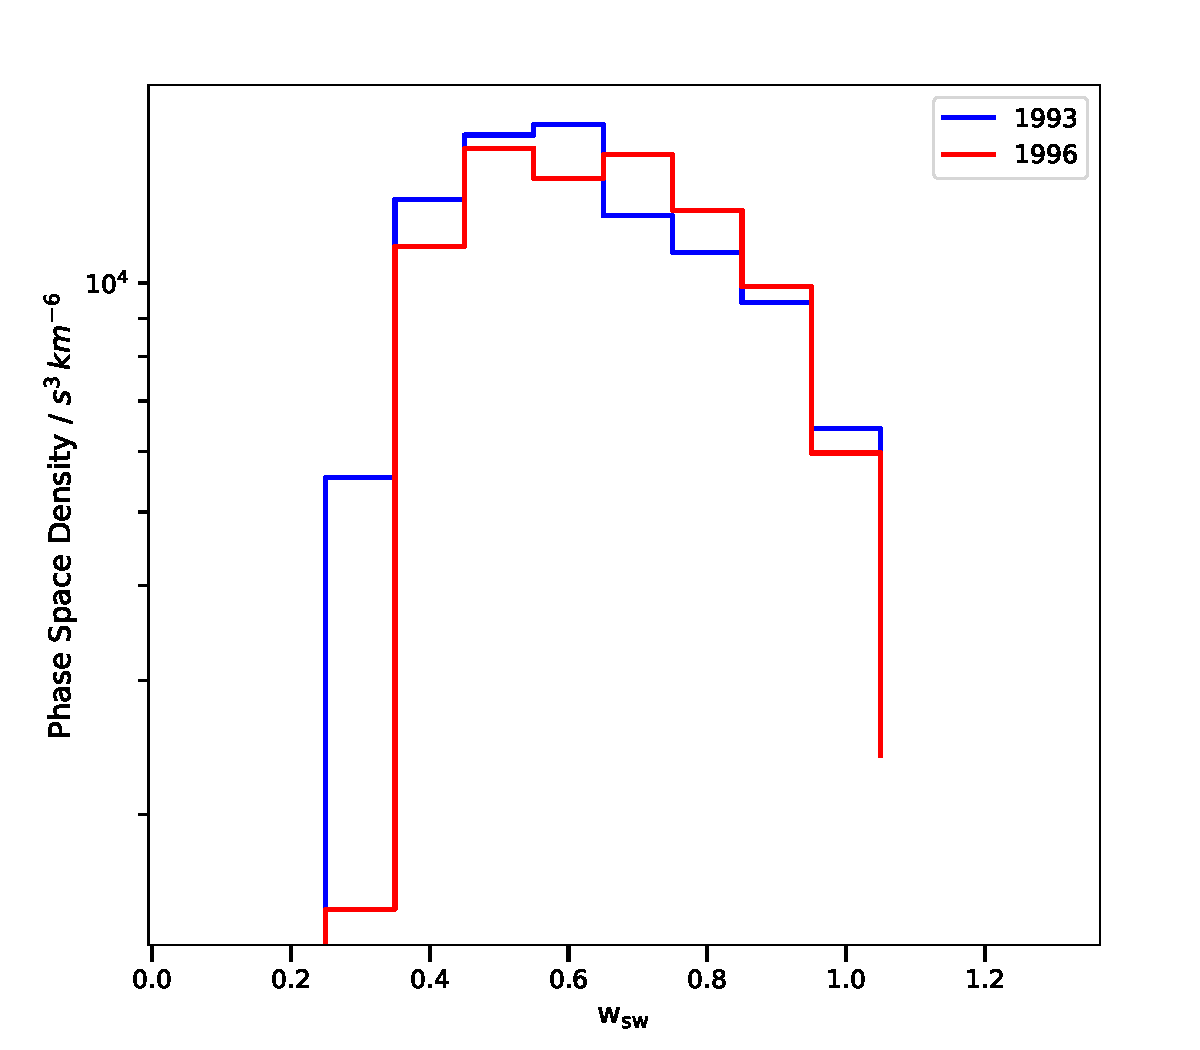
\includegraphics[scale=.38]{Pics/1D.pdf}
	
	\vspace{-0.1cm}
	\begin{center}
		{\tiny $\mathrm{vsw}:760 - 770 \, \mathrm{km\,s^{-1}}$ --
			100 days each in 1994, 1996}
	\end{center}
	\column{4cm}
\end{columns}


\end{frame}



\section{Outlook \& Summary}
%%%

\begin{frame}[plain]{Summary \& Outlook}
\begin{columns}
	\column{8cm}
	\begin{itemize}
		\item $\mathrm{He^+}$ data from Ulysses SWICS
		\item Virtual Detector
		\item Geometrical Effects
		\item Phase Space Normalisation
	\end{itemize}
		\hspace{0.1cm}$\Rightarrow$ 3D measurement of PUI VDF
		\vspace{1cm}
		\hrule
		\vspace{1cm}
{\footnotesize	\begin{itemize}
		\item PUI torus distribution with the IMF
		\item PUI energy diffusion processes

	\end{itemize}}
	\column{5cm}
		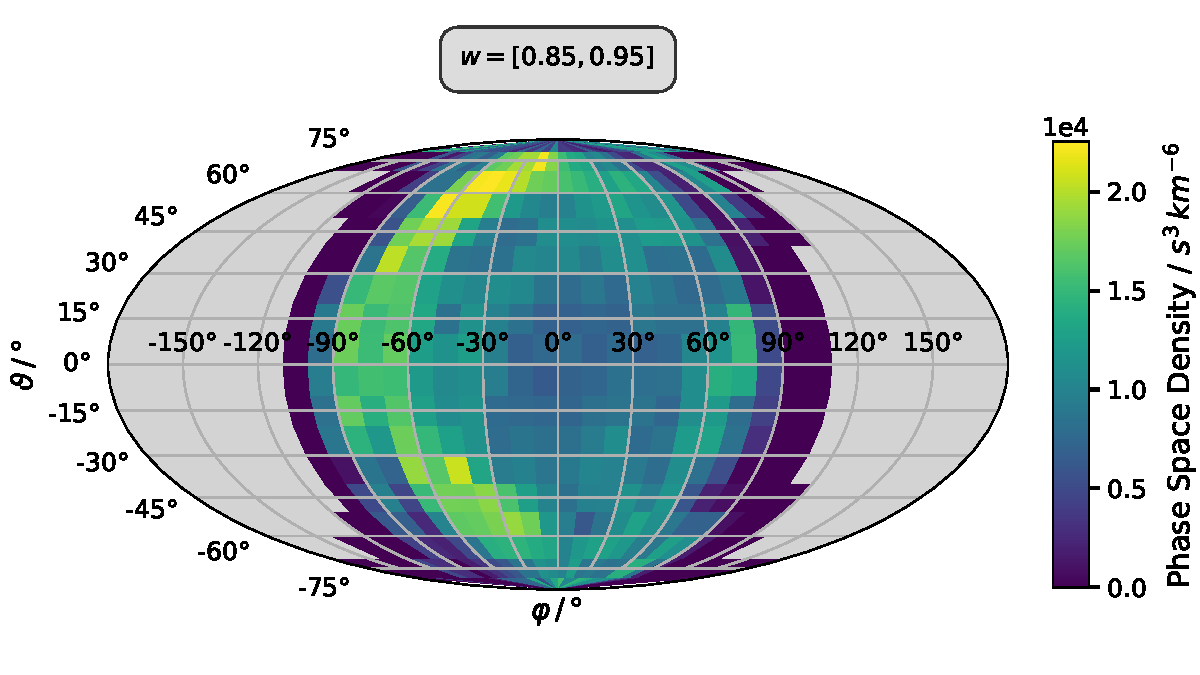
\includegraphics[scale=.2]{Pics/sky_ps.pdf}
		\includegraphics[scale=.21]{Pics/cart_50_ps_R.pdf}
		\includegraphics[scale=.16]{Pics/1D.pdf}
		
\end{columns}


\end{frame}


\begin{frame}[plain]{}
\begin{center}
	{\Huge BACKUP}
\end{center}
\end{frame}

%
%
%
\begin{frame}[plain]{}
	\begin{columns}
	\column[]{5cm}

	\begin{figure}
		\includegraphics[scale=0.23]{Pics/ulysses_instruments.pdf}
		\caption{\tiny{\begin{center}
					\textit{www.cosmos.esa.int, 2019}
		\end{center}}}
	\end{figure}
	
	
	\column[]{6cm}
	\vspace{-1cm}
	\begin{figure}
		\includegraphics[scale=0.45]{Pics/ulysses.jpg}
		\caption{\tiny{\begin{center}
					\textit{McComas et al., 2000}
		\end{center}}}
	\end{figure}
	
	
\end{columns}
\end{frame}


%%%
\begin{frame}{Aspect Angle}
\begin{figure}
	\includegraphics[scale=0.5]{Pics/RTN_AA_angles.pdf}
\end{figure}
\end{frame}


%
%
%
\begin{frame}[plain]{Cartesian Cut: T}
\begin{columns}
	\column{3cm}
	\begin{figure}
		\includegraphics[scale=.7]{Pics/slice_T2.pdf}
	\end{figure}
	\column{6.5cm}
	\begin{figure}
		\includegraphics[scale=.45]{Pics/slice_psd_T.pdf}
	\end{figure}
	\column{.5cm}
\end{columns}
\end{frame}


\begin{frame}[plain]{Cartesian Cut: N}
\begin{columns}
\column{3cm}
\begin{figure}
	\includegraphics[scale=.7]{Pics/slice_N2.pdf}
\end{figure}
\column{6.5cm}
\begin{figure}
	\includegraphics[scale=.45]{Pics/slice_psd_N.pdf}
\end{figure}
\column{.5cm}
\end{columns}
\end{frame}



\begin{frame}[plain]{He$^+$ Data: vsw}
	%\vspace{-1cm}
	\begin{figure}
		\includegraphics[scale=.45]{Pics/vsw_all_years_brw.pdf}
	\end{figure}

\end{frame}

%
%
%

\begin{frame}[plain]
\begin{columns}
	
	\column{4cm}
	\vspace{-0.5cm}
	\begin{figure}
		
		\includegraphics[scale=.28]{Pics/cart_lang_R_counts.pdf}
		\includegraphics[scale=.28]{Pics/cart_lang_R_norm.pdf}
		
	\end{figure}
	\column{6.5cm}
	\begin{figure}
		\includegraphics[scale=.4]{Pics/cart_lang_R_psd.pdf}


 {\scriptsize 		 $\mathrm{vsw} : 740 - 780 \, \mathrm{km\,s^{-1}}$ \\
		 250 days in 1994}

	\end{figure}
	%\column{.5cm}
\end{columns}
\end{frame}

%
%
%
\begin{frame}[plain]{}
\begin{columns}
	\column{7.5cm}
	\begin{figure}
			\includegraphics[scale=.4]{Pics/sky_counts.pdf}
		\includegraphics[scale=.4]{Pics/sky_norm.pdf}
		\end{figure}

	\column{2.5cm}
	\vspace{8cm}
	 {\tiny $\mathrm{vsw}:760 - 780 \, \mathrm{km\,s^{-1}}$ \\
		50 days in 1993}
	
	\end{columns}


\end{frame}


\begin{frame}[plain]{}

	\begin{figure}
		\includegraphics[scale=.6]{Pics/epq_all.pdf}

	\end{figure}
	
\end{frame}

\begin{frame}[plain]{}
\begin{figure}
	\includegraphics[scale=.6]{Pics/cart_50_step-1.pdf}
\end{figure}
\end{frame}

\begin{frame}[plain]{}
\begin{figure}
	\includegraphics[scale=.6]{Pics/cart_50_ps_R.pdf}
\end{figure}
\end{frame}

\begin{frame}[plain]{}
\begin{figure}
	\includegraphics[scale=.6]{Pics/cart_50_R_step1.pdf}
\end{figure}
\end{frame}

\begin{frame}[plain]{}
\begin{figure}
	\includegraphics[scale=.6]{Pics/cart_50_step2.pdf}
\end{figure}
\end{frame}

\begin{frame}[plain]{}
\begin{figure}
	\includegraphics[scale=.6]{Pics/cart_50_step3.pdf}
\end{figure}
\end{frame}

\begin{frame}[plain]{}
\begin{figure}
	\includegraphics[scale=.6]{Pics/cart_50_step4.pdf}
\end{figure}
\end{frame}





%
%
%
\section{Motivation}
\section{kurze Wdh PUIs}
\section{SWICS}

\section{Outlook}
\section{Summary}
%
%
%
\end{document}